\documentclass[a4paper]{article}

\def\npart {II}
\def\nterm {Michaelmas}
\def\nyear {2016}
\def\nlecturer {A. Ashton}
\def\ncourse {Integrable Systems}
\def\nlectures {TT.11}

% Imports
\ifx \nextra \undefined
  \usepackage[pdftex,
    hidelinks,
    pdfauthor={Dexter Chua},
    pdfsubject={Cambridge Maths Notes: Part \npart\ - \ncourse},
    pdftitle={Part \npart\ - \ncourse},
  pdfkeywords={Cambridge Mathematics Maths Math \npart\ \nterm\ \nyear\ \ncourse}]{hyperref}
  \title{Part \npart\ - \ncourse}
\else
  \usepackage[pdftex,
    hidelinks,
    pdfauthor={Dexter Chua},
    pdfsubject={Cambridge Maths Notes: Part \npart\ - \ncourse\ (\nextra)},
    pdftitle={Part \npart\ - \ncourse\ (\nextra)},
  pdfkeywords={Cambridge Mathematics Maths Math \npart\ \nterm\ \nyear\ \ncourse\ \nextra}]{hyperref}

  \title{Part \npart\ - \ncourse \\ {\Large \nextra}}
\fi

\author{Lectured by \nlecturer \\\small Notes taken by Dexter Chua}
\date{\nterm\ \nyear}

\usepackage{alltt}
\usepackage{amsfonts}
\usepackage{amsmath}
\usepackage{amssymb}
\usepackage{amsthm}
\usepackage{booktabs}
\usepackage{caption}
\usepackage{enumitem}
\usepackage{fancyhdr}
\usepackage{graphicx}
\usepackage{mathtools}
\usepackage{microtype}
\usepackage{multirow}
\usepackage{pdflscape}
\usepackage{pgfplots}
\usepackage{siunitx}
\usepackage{tabularx}
\usepackage{tikz}
\usepackage{tkz-euclide}
\usepackage[normalem]{ulem}
\usepackage[all]{xy}

\pgfplotsset{compat=1.12}

\pagestyle{fancyplain}
\lhead{\emph{\nouppercase{\leftmark}}}
\ifx \nextra \undefined
  \rhead{
    \ifnum\thepage=1
    \else
      \npart\ \ncourse
    \fi}
\else
  \rhead{
    \ifnum\thepage=1
    \else
      \npart\ \ncourse\ (\nextra)
    \fi}
\fi
\usetikzlibrary{arrows}
\usetikzlibrary{decorations.markings}
\usetikzlibrary{decorations.pathmorphing}
\usetikzlibrary{positioning}
\usetikzlibrary{fadings}
\usetikzlibrary{intersections}
\usetikzlibrary{cd}

\newcommand*{\Cdot}{\raisebox{-0.25ex}{\scalebox{1.5}{$\cdot$}}}
\newcommand {\pd}[2][ ]{
  \ifx #1 { }
    \frac{\partial}{\partial #2}
  \else
    \frac{\partial^{#1}}{\partial #2^{#1}}
  \fi
}

% Theorems
\theoremstyle{definition}
\newtheorem*{aim}{Aim}
\newtheorem*{axiom}{Axiom}
\newtheorem*{claim}{Claim}
\newtheorem*{cor}{Corollary}
\newtheorem*{defi}{Definition}
\newtheorem*{eg}{Example}
\newtheorem*{fact}{Fact}
\newtheorem*{law}{Law}
\newtheorem*{lemma}{Lemma}
\newtheorem*{notation}{Notation}
\newtheorem*{prop}{Proposition}
\newtheorem*{thm}{Theorem}

\renewcommand{\labelitemi}{--}
\renewcommand{\labelitemii}{$\circ$}
\renewcommand{\labelenumi}{(\roman{*})}

\let\stdsection\section
\renewcommand\section{\newpage\stdsection}

% Strike through
\def\st{\bgroup \ULdepth=-.55ex \ULset}

% Maths symbols
\newcommand{\bra}{\langle}
\newcommand{\ket}{\rangle}

\newcommand{\N}{\mathbb{N}}
\newcommand{\Z}{\mathbb{Z}}
\newcommand{\Q}{\mathbb{Q}}
\renewcommand{\H}{\mathbb{H}}
\newcommand{\R}{\mathbb{R}}
\newcommand{\C}{\mathbb{C}}
\newcommand{\Prob}{\mathbb{P}}
\renewcommand{\P}{\mathbb{P}}
\newcommand{\E}{\mathbb{E}}
\newcommand{\F}{\mathbb{F}}
\newcommand{\cU}{\mathcal{U}}
\newcommand{\RP}{\mathbb{RP}}
\newcommand{\CP}{\mathbb{CP}}

\newcommand{\ph}{\,\cdot\,}

\DeclareMathOperator{\sech}{sech}
\DeclareMathOperator{\cosech}{cosech}
\DeclareMathOperator{\cosec}{cosec}

\DeclareMathOperator{\covol}{covol}
\DeclareMathOperator{\vol}{vol}

\let\Im\relax
\let\Re\relax
\DeclareMathOperator{\Im}{Im}
\DeclareMathOperator{\Re}{Re}
\DeclareMathOperator{\im}{im}
\DeclareMathOperator{\image}{image}
\DeclareMathOperator{\Ann}{Ann}

\DeclareMathOperator*{\res}{res}
\DeclareMathOperator{\Res}{Res}
\DeclareMathOperator{\Ind}{Ind}

\DeclareMathOperator{\tr}{tr}
\DeclareMathOperator{\diag}{diag}
\DeclareMathOperator{\rank}{rank}
\DeclareMathOperator{\card}{card}
\DeclareMathOperator{\spn}{span}
\DeclareMathOperator{\adj}{adj}

\DeclareMathOperator{\erf}{erf}
\DeclareMathOperator{\erfc}{erfc}

\DeclareMathOperator{\ord}{ord}
\DeclareMathOperator{\Sym}{Sym}

\DeclareMathOperator{\sgn}{sgn}
\DeclareMathOperator{\orb}{orb}
\DeclareMathOperator{\stab}{stab}
\DeclareMathOperator{\ccl}{ccl}

\DeclareMathOperator{\lcm}{lcm}
\DeclareMathOperator{\hcf}{hcf}

\DeclareMathOperator{\Int}{Int}
\DeclareMathOperator{\id}{id}

\DeclareMathOperator{\betaD}{beta}
\DeclareMathOperator{\gammaD}{gamma}
\DeclareMathOperator{\Poisson}{Poisson}
\DeclareMathOperator{\binomial}{binomial}
\DeclareMathOperator{\multinomial}{multinomial}
\DeclareMathOperator{\Bernoulli}{Bernoulli}
\DeclareMathOperator{\like}{like}

\DeclareMathOperator{\var}{var}
\DeclareMathOperator{\cov}{cov}
\DeclareMathOperator{\bias}{bias}
\DeclareMathOperator{\mse}{mse}
\DeclareMathOperator{\corr}{corr}

\DeclareMathOperator{\otp}{otp}
\DeclareMathOperator{\dom}{dom}

\DeclareMathOperator{\Root}{Root}
\DeclareMathOperator{\supp}{supp}
\DeclareMathOperator{\rel}{rel}
\DeclareMathOperator{\Hom}{Hom}
\DeclareMathOperator{\Aut}{Aut}
\DeclareMathOperator{\Gal}{Gal}
\DeclareMathOperator{\Mat}{Mat}
\DeclareMathOperator{\End}{End}
\DeclareMathOperator{\Char}{char}
\DeclareMathOperator{\ev}{ev}
\DeclareMathOperator{\St}{St}
\DeclareMathOperator{\Lk}{Lk}
\DeclareMathOperator{\disc}{disc}
\DeclareMathOperator{\Isom}{Isom}
\DeclareMathOperator{\length}{length}
\DeclareMathOperator{\energy}{energy}
\DeclareMathOperator{\area}{area}
\DeclareMathOperator{\Syl}{Syl}
\DeclareMathOperator{\cl}{cl}
\DeclareMathOperator{\fix}{fix}

\newcommand{\GL}{\mathrm{GL}}
\newcommand{\SL}{\mathrm{SL}}
\newcommand{\PGL}{\mathrm{PGL}}
\newcommand{\PSL}{\mathrm{PSL}}
\newcommand{\PSU}{\mathrm{PSU}}
\newcommand{\Or}{\mathrm{O}}
\newcommand{\SO}{\mathrm{SO}}
\newcommand{\U}{\mathrm{U}}
\newcommand{\SU}{\mathrm{SU}}

\renewcommand{\d}{\mathrm{d}}
\newcommand{\D}{\mathrm{D}}

\tikzset{->/.style = {decoration={markings,
                                  mark=at position 1 with {\arrow[scale=2]{latex'}}},
                      postaction={decorate}}}
\tikzset{<-/.style = {decoration={markings,
                                  mark=at position 0 with {\arrowreversed[scale=2]{latex'}}},
                      postaction={decorate}}}
\tikzset{<->/.style = {decoration={markings,
                                   mark=at position 0 with {\arrowreversed[scale=2]{latex'}},
                                   mark=at position 1 with {\arrow[scale=2]{latex'}}},
                       postaction={decorate}}}
\tikzset{->-/.style = {decoration={markings,
                                   mark=at position #1 with {\arrow[scale=2]{latex'}}},
                       postaction={decorate}}}
\tikzset{-<-/.style = {decoration={markings,
                                   mark=at position #1 with {\arrowreversed[scale=2]{latex'}}},
                       postaction={decorate}}}

\tikzset{circ/.style = {fill, circle, inner sep = 0, minimum size = 3}}
\tikzset{mstate/.style={circle, draw, blue, text=black, minimum width=0.7cm}}

\definecolor{mblue}{rgb}{0.2, 0.3, 0.8}
\definecolor{morange}{rgb}{1, 0.5, 0}
\definecolor{mgreen}{rgb}{0.1, 0.4, 0.2}
\definecolor{mred}{rgb}{0.5, 0, 0}

\def\drawcirculararc(#1,#2)(#3,#4)(#5,#6){%
    \pgfmathsetmacro\cA{(#1*#1+#2*#2-#3*#3-#4*#4)/2}%
    \pgfmathsetmacro\cB{(#1*#1+#2*#2-#5*#5-#6*#6)/2}%
    \pgfmathsetmacro\cy{(\cB*(#1-#3)-\cA*(#1-#5))/%
                        ((#2-#6)*(#1-#3)-(#2-#4)*(#1-#5))}%
    \pgfmathsetmacro\cx{(\cA-\cy*(#2-#4))/(#1-#3)}%
    \pgfmathsetmacro\cr{sqrt((#1-\cx)*(#1-\cx)+(#2-\cy)*(#2-\cy))}%
    \pgfmathsetmacro\cA{atan2(#2-\cy,#1-\cx)}%
    \pgfmathsetmacro\cB{atan2(#6-\cy,#5-\cx)}%
    \pgfmathparse{\cB<\cA}%
    \ifnum\pgfmathresult=1
        \pgfmathsetmacro\cB{\cB+360}%
    \fi
    \draw (#1,#2) arc (\cA:\cB:\cr);%
}
\newcommand\getCoord[3]{\newdimen{#1}\newdimen{#2}\pgfextractx{#1}{\pgfpointanchor{#3}{center}}\pgfextracty{#2}{\pgfpointanchor{#3}{center}}}

\def\Xint#1{\mathchoice
   {\XXint\displaystyle\textstyle{#1}}%
   {\XXint\textstyle\scriptstyle{#1}}%
   {\XXint\scriptstyle\scriptscriptstyle{#1}}%
   {\XXint\scriptscriptstyle\scriptscriptstyle{#1}}%
   \!\int}
\def\XXint#1#2#3{{\setbox0=\hbox{$#1{#2#3}{\int}$}
     \vcenter{\hbox{$#2#3$}}\kern-.5\wd0}}
\def\ddashint{\Xint=}
\def\dashint{\Xint-}


\begin{document}
\maketitle
{\small
\noindent\emph{Part IB Methods, and Complex Methods or Complex Analysis are essential; Part II Classical Dynamics is desirable.}

\vspace{10pt}
\noindent Integrability of ordinary differential equations: Hamiltonian systems and the Arnol'd--Liouville Theorem (sketch of proof). Examples.\hspace*{\fill}[3]

\vspace{5pt}
\noindent Integrability of partial differential equations: The rich mathematical structure and the universality of the integrable nonlinear partial differential equations (Korteweg-de Vries, sine-Gordon). Backlund transformations and soliton solutions.\hspace*{\fill}[2]

\vspace{5pt}
\noindent The inverse scattering method: Lax pairs. The inverse scattering method for the KdV equation, and other integrable PDEs. Multi soliton solutions. Zero curvature representation. \hspace*{\fill}[6]

\vspace{5pt}
\noindent Hamiltonian formulation of soliton equations.\hspace*{\fill}[2]

\vspace{5pt}
\noindent Painleve equations and Lie symmetries: Symmetries of differential equations, the ODE reductions of certain integrable nonlinear PDEs, Painleve equations.\hspace*{\fill}[3]%
}

\tableofcontents
\setcounter{section}{-1}
\section{Introduction}
What is an integrable system? Unfortunately, an integrable system is a something mathematicians have not yet managed to define properly. Intuitively, an integrable system is a differential equation we can ``integrate up'' directly. While in theory, integrable systems should be very rare, it happens that in nature, a lot of systems happen to be integrable. By exploiting the fact that they are integrable, we can solve them much more easily.

\section{Integrability of ODE's}
\subsection{Vector fields and flow maps}
For a vector field $\mathbf{V}: \R^m \to \R^m$, consider a differential equation for $\mathbf{x}(t) \in \R^m$,
\[
  \dot{\mathbf{x}} = \mathbf{V}(\mathbf{x}),\quad \mathbf{x}(0) = \mathbf{x}_0.
\]
In this course, we will assume the vector field $\mathbf{V}$ is ``nice'', in the sense that the solutions always exist and are unique, and are infinitely differentiable.

It is convenient to write the solution as
\[
  \mathbf{x}(t) = g^t \mathbf{x}_0,
\]
where $g^t: \R^m \to \R^m$ is called the \emph{flow map}. This has some nice properties:
\begin{prop}\leavevmode
  \begin{enumerate}
    \item $g_0 = \id$
    \item $g^{t + s} = g^t g^s$
    \item $(g^{t})^{-1} = g^{-t}$
  \end{enumerate}
\end{prop}
The proofs are left for the first example sheet.

We say that $\mathbf{V}$ is the \emph{infinitesimal generator} of the flow $g^t$. This is because
\[
  \mathbf{x}(\varepsilon) = g^\varepsilon \mathbf{x}_0 = \mathbf{x}(0) + \varepsilon \dot{\mathbf{x}}(0) + o(\varepsilon) = \mathbf{x}_0 + \varepsilon \mathbf{V}(\mathbf{x}_0) + o(\varepsilon).
\]
For two vector fields $\mathbf{V}_1, \mathbf{V}_2: \R^m \to \R^m$ which generate flows $g_1^t$ and $g_2^s$, we define the third vector field, the commutator, by
\[
  [\mathbf{V}_1, \mathbf{V}_2] = \left(\mathbf{V}_1 \cdot \frac{\partial}{\partial \mathbf{x}}\right) \mathbf{V}_2 - \left(\mathbf{V}_2 \cdot \frac{\partial}{\partial \mathbf{x}}\right) \mathbf{V}_1,
\]
where we write
\[
  \frac{\partial}{\partial \mathbf{x}} = \left(\frac{\partial}{\partial x_1}, \cdots, \frac{\partial}{\partial x_n}\right)^T.
\]
More explicitly, the $i$th component
\[
  [\mathbf{V}_1, \mathbf{V}_2]_i = \sum_{j = 1}^m (\mathbf{v}_1)_j \frac{\partial}{\partial x_j} (\mathbf{v}_2)_i - (\mathbf{v}_2)_j \frac{\partial}{\partial x_j} (\mathbf{v}_1)_i
\]
This is a very important concept, because we have
\begin{prop}
  \[
    [\mathbf{V}_1, \mathbf{V}_2] = 0 \Leftrightarrow g_1^t g_2^s = g_2^s g_1^t.
  \]
\end{prop}
This will be shown in the first example sheet.

Thus, to figure out if two flows commute, it suffices to check if their infinitesimal generates commutative.
\subsection{Phase space and Poisson brackets}
In this section, we are interested in dynamical problems on a $2n$-dimensional \emph{phase space} $M$. Points on $M$ are described by coordinates
\[
  (\mathbf{q}, \mathbf{p}) = (q_1, \cdots, q_n, p_1, \cdots, p_n).
\]
We tend to think of the $q_i$ are ``generalized positions'' of particles, and the $p_n$ as the ``generalized momentum'' coordinates. We will often write
\[
  \mathbf{x} = (\mathbf{q}, \mathbf{p})^T.
\]
We introduce a $2n \times 2n$ anti-symmetric matrix
\[
  J =
  \begin{pmatrix}
    0 & I_n\\
    -I_n & 0
  \end{pmatrix}.
\]
We are now going to define a \emph{Poisson bracket}.

\begin{defi}[Poisson bracket]
  For any two functions $f, g: M \to \R$, we define the \emph{Poisson bracket} by
  \[
    \{f, g\} = \frac{\partial f}{\partial \mathbf{x}} J \frac{\partial g}{\partial \mathbf{x}} = \frac{\partial f}{\partial \mathbf{q}} \cdot \frac{\partial g}{\partial \mathbf{p}} - \frac{\partial f}{\partial \mathbf{p}} \cdot \frac{\partial g}{\partial \mathbf{q}}.
  \]
\end{defi}

This has some obvious and not-so-obvious properties:
\begin{prop}\leavevmode
  \begin{enumerate}
    \item This is linear in each argument.
    \item This is antisymmetric, ie. $\{f, g\} = - \{g, f\}$.
    \item Leibniz property: $\{f, gh\} = \{f, g\}h + \{f, h\} g$.
    \item Jacobi identity: $\{f, \{g, h\}\} + \{g, \{h, f\}\} + \{h, \{f, g\}\} = 0$.
    \item
      \[
        \{q_i, q_j\} = \{p_i, p_j\} = 0,\quad \{q_i, p_j\} = \delta_{ij}.
      \]
  \end{enumerate}
\end{prop}

\subsection{Hamiltonian dynamics}
We will be interested in problems on $M$ of the following form:
\begin{defi}[Hamilton's equation]
  \emph{Hamilton's equation} is an equation of the form
  \[
    \dot{\mathbf{q}} = \frac{\partial H}{\partial \mathbf{p}},\quad \dot{\mathbf{p}} = -\frac{\partial H}{\partial \mathbf{q}}\tag{$*$}
  \]
  For some function $H: M \to \R$ called the \emph{Hamiltonian}.
\end{defi}
Just as we think of $\mathbf{q}$ and $\mathbf{p}$ as generalized position and momentum, we tend to think of $H$ as generalized energy.

Note that $(*)$ can be written as
\[
  \dot{\mathbf{x}} = J \frac{\partial H}{\partial \mathbf{x}}.
\]
Compare this to the equation
\[
  \dot{\mathbf{x}} = \mathbf{V}(\mathbf{x}), \quad \mathbf{x}(0) = \mathbf{x}_0.
\]
Assuming that $\mathbf{x}$ evolves according to Hamilton's equations, if $f: M \to \R$ is a smooth function, then by the chain rule, we have
\begin{align*}
  \frac{\d f}{\d t} &= \frac{\d}{\d t} f(\mathbf{q}(t), \mathbf{p}(t))\\
  &= \frac{\partial f}{\partial \mathbf{q}} \cdot \dot{\mathbf{q}} + \frac{\partial f}{\partial \mathbf{p}} \cdot \dot{\mathbf{p}}\\
  &= \frac{\partial f}{\partial \mathbf{q}} \cdot \frac{\partial H}{\partial \mathbf{p}} - \frac{\partial f}{\partial \mathbf{p}} \cdot \frac{\partial H}{\partial \mathbf{q}} \\
  &= \{f, H\}.
\end{align*}
In particular, we have
\[
  \frac{\d H}{\d t} = \{H, H\} = 0.
\]
So the Hamiltonian is constant!
\begin{eg}
  Consider a particle (of unit mass) with position $\mathbf{q} = (q_1, q_2, q_3)$ (in Cartesian coordinates) moving under the influence of a potential $U(\mathbf{q})$. By Newton's second law, we have
  \[
    \ddot{\mathbf{q}} = -\frac{\partial U}{\partial \mathbf{q}}.
  \]
  This is actually a Hamiltonian system. We define the momentum variables by
  \[
    p_i = \dot{q}_i,
  \]
  then we have
  \[
    \dot{\mathbf{x}} =
    \begin{pmatrix}
      \dot{\mathbf{q}}
      \dot{\mathbf{p}}
    \end{pmatrix}
    =
    \begin{pmatrix}
      \mathbf{p}\\
      -\frac{\partial U}{\partial \mathbf{q}}
    \end{pmatrix}
    = J \frac{\partial H}{\partial \mathbf{x}},
  \]
  with
  \[
    H = \frac{1}{2} \abs{\mathbf{p}}^2 + U(\mathbf{q}).
  \]
  This is just the usual energy! Indeed, we have
  \[
    \frac{\partial H}{\partial \mathbf{p}} = \mathbf{p},\quad \frac{\partial H}{\partial \mathbf{q}} = \frac{\partial H}{\partial \mathbf{q}}.
  \]
\end{eg}

\begin{defi}[Hamiltonian vector field]\index{Hamiltonian vector field}
  Given a Hamiltonian function $H$, the \emph{Hamiltonian vector field} is given by
  \[
    \mathbf{V}_H = J \frac{\partial H}{\partial \mathbf{x}}.
  \]
\end{defi}

We then see that the Hamiltonian vector field generates the Hamiltonian flow. More generally, for any $f: M \to \R$, we call
\[
  \mathbf{V}_f = J \frac{\partial f}{\partial \mathbf{x}}.
\]
This is the Hamiltonian vector field with respect to $f$ and $g$.

\begin{prop}
  We have
  \[
    [V_\mathbf{f}, V_\mathbf{g}] = - \mathbf{V}_{\{f, g\}}.
  \]
\end{prop}

\begin{proof}
  See first example sheet. % Fill in
\end{proof}

\begin{defi}[First integral]\index{first integral}
  Given a phase space $M$ with a Hamiltonian $H$, we call $f: M \to \R$ a \emph{first integral} of the Hamiltonian system if
  \[
    \{f, H\} = 0.
  \]
\end{defi}
The reason for the term ``first integral'' is historical --- when we solve a differential equation, we integrate the equation. Every time we integrate it, we obtain a new constant. And the first constant we obtain when we integrate is known as the first integral. However, for our purposes, we can just as well think of it as a constant of motion.

\begin{eg}
  Consider the two-body problem --- the Sun is fixed at the origin, and a planet has Cartesian coordinates $\mathbf{q} = (q_1, q_2, q_3)$. The equation of motion will be
  \[
    \ddot{\mathbf{q}} = - \frac{\mathbf{q}}{|\mathbf{q}|^3}.
  \]
  This is equivalent to the Hamiltonian system $\mathbf{p} = \dot{\mathbf{q}}$, with
  \[
    H = \frac{1}{2} |\mathbf{p}|^2 - \frac{1}{|\mathbf{q}|}.
  \]
  We have an angular momentum given by
  \[
    \mathbf{L} = \mathbf{q} \wedge \mathbf{p}.
  \]
  Working with coordinates, we have
  \[
    L_i = \varepsilon_{ijk} q_j p_k.
  \]
  We then have
  \begin{align*}
    \{L_i, H\} &= \frac{\partial L_i}{\partial q_\ell}\frac{\partial H}{\partial p_\ell} - \frac{\partial L_i}{\partial p_\ell} \frac{\partial H}{\partial q_\ell}\\
    &= \varepsilon_{ijk} \left(p_k \delta_{\ell j}p_\ell + \frac{q_j q_k}{|\mathbf{q}|^3}\right)\\
    &= \varepsilon_{ijk} \left(p_k p_j + \frac{q_j q_k}{|\mathbf{q}|^3}\right)\\
    &= 0,
  \end{align*}
  where we know the thing vanishes because we contracted a symmetric tensor with an antisymmetric one. So this is a first integral.

  Less interestingly, we know $H$ is also a first integral. In general, some Hamiltonian have many many first integrals.
\end{eg}

\begin{defi}[Involution]\index{involution}
  We say that two first integrals $F, G$ are in \emph{involution} if $\{F, G\} = 0$ (so $F$ and $G$ ``\emph{Poisson commute}'').
\end{defi}

\begin{defi}[Independent first integrals]\index{independent first integrals}
  A collection of functions $f_i: M \to \R$ are independent if at each $\mathbf{x} \in M$, the vectors $\frac{\partial f_i}{\partial \mathbf{x}}$ for $i = 1, \cdots, n$ are independent.
\end{defi}

\begin{defi}[Integrable system]\index{integrable system}
  A $2n$-dimensional Hamiltonian system $(M, H)$ is \emph{integrable} if there exists $n$ first integrals $\{f_i\}_{i = 1}^n$ that are independent and in involution (ie. $\{f_i, f_j\} = 0$ for all $i, j$).
\end{defi}
The word independent is very important, or else people will cheat, eg. take $H, 2H, e^H, H^2, \cdots$.

\begin{cor}
  Two-dimensional Hamiltonian systems are always integrable.
\end{cor}

We are now ready for the main section.
%\section{Action-angle coordinates and the Arnold-Liouville theorem}
\section{The Arnold-Liouville theorem}
Consider the Hamiltonian system
\[
  \dot{\mathbf{q}} = \frac{\partial H}{\partial \mathbf{q}},\quad \mathbf{p} = -\frac{\partial H}{\partial \mathbf{q}}.
\]
We do not expect a general coordinate change $(\mathbf{q}, \mathbf{p}) \mapsto (\mathbf{Q}(\mathbf{q}, \mathbf{q}), \mathbf{P}(\mathbf{q}, \mathbf{p}))$ to hold the form of Hamilton's equations, ie. we will no longer have
\[
  \dot{\mathbf{Q}} = \frac{\partial \tilde{H}}{\partial \mathbf{P}},\quad \dot{\mathbf{P}} = -\frac{\partial \tilde{H}}{\partial \mathbf{Q}},
\]
where $\tilde{H}(\mathbf{Q}, \mathbf{P}) = H(\mathbf{q}, \mathbf{p})$.

If we write $\mathbf{x} = (\mathbf{q}, \mathbf{p})$ and $\mathbf{y} = (\mathbf{Q}, \mathbf{P})$, then this is equivalent to asking if
\[
  \dot{\mathbf{x}} = J \frac{\partial H}{\partial \mathbf{x}} \quad\Rightarrow\quad \dot{\mathbf{y}} = J \frac{\partial \tilde{H}}{ \partial \mathbf{y}}.
\]
For example, if we just swap $\mathbf{p}$ and $\mathbf{q}$ around, the form of the equation changes (namely the signs go in the wrong place).

\begin{defi}[Canonical transformation]\index{canonical transformation}
  A coordinate change $(\mathbf{q}, \mathbf{p}) \mapsto (\mathbf{Q}, \mathbf{P})$ is called \emph{canonical} if it leaves Hamilton's equations invariant, ie. we have
  \[
    \dot{\mathbf{Q}} = \frac{\partial \tilde{H}}{\partial \mathbf{P}},\quad \dot{\mathbf{P}} = -\frac{\partial \tilde{H}}{\partial \mathbf{Q}},
  \]
\end{defi}

\begin{eg}
  The simplest possible case of a canonical transformation is a linear transformation. Consider a linear change of coordinates given by
  \[
    \mathbf{x} \mapsto \mathbf{y}(\mathbf{x}) = A\mathbf{x}.
  \]
  We claim that this is canonical iff $AJA^t = J$, ie. that $A$ is \term{symplectic}.

  Indeed, by linearity, we have
  \[
    \dot{\mathbf{y}} = A\dot{\mathbf{x}} = AJ\frac{\partial H}{\mathbf{x}}.
  \]
  Setting $\tilde{\mathbf{H}}(\mathbf{y} = H(\mathbf{x})$, we have
  \[
    \frac{\partial H}{\partial x_i} = \frac{\partial y_j}{\partial x_i} \frac{\partial \tilde{H}(\mathbf{y})}{\partial y_j} = A_{ji} \frac{\partial \tilde{H}(\mathbf{y})}{\partial y_j}(\mathbf{y}) = \left[A^T \frac{\partial \tilde{H}}{\partial \mathbf{y}}\right]_i.
  \]
  Putting this back in, we have
  \[
    \dot{\mathbf{y}} = AJA^T \frac{\partial\tilde{H}}{\partial \mathbf{y}}.
  \]
  So $\mathbf{y} \mapsto \mathbf{y}(\mathbf{x})$ is canonical if $J = AJA^T$.
\end{eg}

What about more general cases? Recall from IB Analysis II that a map is differentiable if it is ``locally linear''. Now Hamilton's equations are purely local equations, so we might expect the following:
\begin{prop}
  A map $\mathbf{x} \mapsto \mathbf{y}(\mathbf{x})$ is canonical iff $D\mathbf{y}$ is symplectic, ie.
  \[
    D\mathbf{y} J (D\mathbf{y})^T = J.
  \]
\end{prop}

Now could we find a canonical transformation $(\mathbf{q}, \mathbf{p}) \mapsto (\mathbf{Q}, \mathbf{P})$ such that $\tilde{H}$ depends only on $\mathbf{P}$. If this happened, then Hamilton's equations reduce to
\[
  \dot{\mathbf{Q}} = \frac{\partial \tilde{H}}{\partial \mathbf{P}}(\mathbf{P}),\quad \dot{\mathbf{P}} = -\frac{\partial \tilde{H}}{\partial \mathbf{Q}} = 0.
\]
So $\mathbf{P}(t) = \mathbf{P}_0$ is a constant. Since the right hand side of the first equation depends only on $\mathbf{P}$, we find that $\dot{\mathbf{Q}}$ is also constant! So $\mathbf{Q} = \mathbf{Q}_0 + \Omega t$, where
\[
  \Omega = \frac{\partial \tilde{H}}{\partial \mathbf{P}} (\mathbf{P}_0).
\]
So if we could find a good canonical transformation, the solution falls out easily! It turns out that if a system is integrable, then we can indeed find such coordinates.

We are now going to prove the Arnold-Liouville theorem. Before we do that in full generality, we first do it in a specific case, and see how the proof actually works out.

\begin{eg}
  Consider the harmonic oscillator with Hamiltonian
  \[
    H(q, p) = \frac{1}{2}p^2 + \frac{1}{2}\omega^2 q^2.
  \]
  Since is a 2-dimensional system, so we only need a single first integral. Since $H$ is a first integral for trivial reasons, this is an integrable Hamiltonian system.

  We can actually draw the lines on which $H$ is constant --- they are just ellipses:
  \begin{center}
    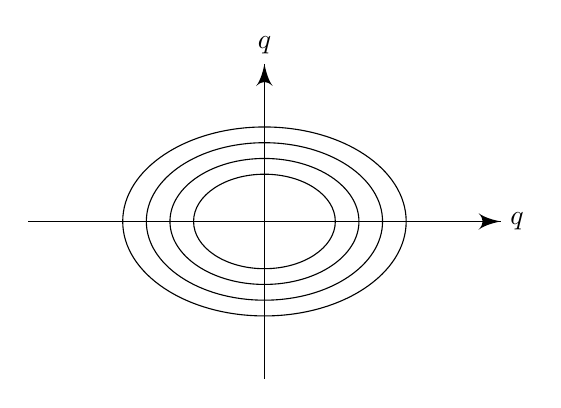
\begin{tikzpicture}
      \draw [->] (-3, 0) -- (3, 0) node [right] {$q$};
      \draw [->] (0, -2) -- (0, 2) node [above] {$q$};

      \foreach \x in {0.6, 0.8, 1, 1.2} {
        \begin{scope}[scale=\x]
          \draw ellipse (1.5 and 1);
        \end{scope}
      }
    \end{tikzpicture}
  \end{center}
  We note that the ellipses are homeomorphic to $S^1$. Now we introduce the coordinate transformation $(q, p) \mapsto (\phi, I)$, defined by
  \[
    q = \sqrt{\frac{2I}{\omega}} \sin \phi,\quad p = \sqrt{2I\omega} \cos \phi,
  \]
  For the purpose of this example, we can suppose we obtained this formula through divine inspiration. However, in the Arnold-Liouville theorem, we will provide a general way of coming up with these formulas.

  We can manually show that this transformation is canonical (it is actually easier to show that the inverse map $(\phi, I) \mapsto (q, p)$ is canonical). We also have that
  \[
    \tilde{H}(\phi, I) = H(q(\phi, I), p(\phi, I)) = \omega I.
  \]
  This is really nice. There is no $\phi$! Now Hamilton's equations become
  \[
    \dot\phi = \frac{\partial \tilde{H}}{ \partial I} = \omega,\quad \dot{I} = -\frac{\partial \tilde{H}}{\partial \phi} = 0.
  \]
  We can integrate up to obtain
  \[
    \phi(t) = \phi_0 + \omega t,\quad I(t) = I_0.
  \]
  It is fun to consider the integral along paths of constant $H$:
  \begin{align*}
    \frac{1}{2\pi}\oint p \;\d q &= \frac{1}{2\pi} \int_0^{2\pi}p(\phi, I) \left(\frac{\partial q}{\partial \phi} \;\d \phi + \frac{\partial q}{\partial I} \;\d I\right)\\
    &= \frac{1}{2\pi} \int_0^{2\pi}p(\phi, I) \left(\frac{\partial q}{\partial \phi} \;\d \phi\right)\\
    &= \frac{1}{2\pi} \int_0^{2\pi} \sqrt{\frac{2I}{\omega}}\sqrt{2I\omega} \cos^2 \phi \;\d \phi\\
    &= I
  \end{align*}
  This is interesting. We didn't know how we obtained $I$, but in fact we can obtain it by performing an integral like this.
\end{eg}
There are two things to take away from this.
\begin{enumerate}
  \item The motion takes place in $S^1$
  \item We got $I$ by performing $\frac{1}{2\pi}\oint p \;\d q$.
\end{enumerate}
These two ideas are essentially what we are going to prove for general Hamiltonian system.

% insert something about generating functions

\begin{thm}[Arnold-Liouville theorem]\index{Arnold-Liouville theorem}
  We let $(M, H)$ be an integrable $2n$-dimensional Hamiltonian system with independent, involutive first integrals $f_1, \cdots, f_n$, where $f_1 = H$. For any fixed $\mathbf{c} \in \R^n$, we set
  \[
    M_\mathbf{c} = \{(\mathbf{q}, \mathbf{p}) \in M: f_i(\mathbf{q}, \mathbf{p}) = c_i, i =1 , \cdots, n\}.
  \]
  Then
  \begin{enumerate}
    \item $M_\mathbf{c}$ is a smooth $n$-dimensional surface in $M$. If $M_\mathbf{c}$ is compact and connected, then it is diffeomorphic to
      \[
        T^n = S^1 \times \cdots \times S^1.
      \]
    \item (\ldots) % fill in
  \end{enumerate}
\end{thm}

\begin{proof}[Proof sketch]
  We first show that $M_\mathbf{c}$ is smooth and $n$-dimensional. We will handwave through this part. The proper proof follows easily from techniques found in IID Differential geometry using the implicit function theorem. We know $M_\mathbf{c}$ is a surface defined by $n$ constraints, while the whole phase space $M$ has $2n$ degrees of freedom. So the remaining number of degrees of freedom on $M_\mathbf{c}$ is $n$. The key that makes this work is that the constraints are independent, which is the condition that allows us to apply the implicit function theorem.

  We now show that $M_\mathbf{c}$ is diffeomorphic to the torus if it is compact and connected. Consider the Hamiltonian vector fields defined by
  \[
    \mathbf{V}_{f_i} = J \frac{\partial f_i}{\partial \mathbf{x}}.
  \]
  We claim that these are \emph{tangent} to the surface $M_\mathbf{c}$. Indeed, we want to see if any of the $\{f_j\}$ change in the direction of $\mathbf{V}_{f_i}$. We can compute
  \[
    \left(\mathbf{V}_{f_i} \cdot \frac{\partial}{\partial \mathbf{x}}\right)f_j = \frac{\partial f_j}{\partial \mathbf{x}} J \frac{\partial f_i}{\partial \mathbf{x}} = \{f_j, f_i\} = 0.
  \]
  Since this vanishes, we know that $\mathbf{V}_{f_i}$ is a tangent a tangent to the surface. So the flow maps $\{g_i\}$ map $M_\mathbf{c}$ to itself. Also, we know that the flow maps commute. Indeed, we can compute
  \[
    [\mathbf{V}_{f_i}, \mathbf{V}_{f_j}] = -\mathbf{V}_{\{f_i, f_j\}} = -\mathbf{V}_{0} = 0.
  \]
  So we have a whole bunch of commuting flow maps from $M_\mathbf{c}$ to itself. We set
  \[
    g^\mathbf{t} = g_1^{t_1} g_2^{t_2} \cdots g_n^{t_n},
  \]
  where $\mathbf{t} \in \R^n$. Then because of commutativity, we have
  \[
    g^{\mathbf{t}_1 + \mathbf{t}_2} = g^{\mathbf{t}_1}g^{\mathbf{t}_2}.
  \]
  So this is gives a group action of $\R^n$ on the surface $M_\mathbf{c}$. We fix $\mathbf{x} \in M_\mathbf{c}$. We define
  \[
    \stab(\mathbf{x}) = \{\mathbf{t} \in \R^n: g^\mathbf{t}\mathbf{x} = \mathbf{x}\}.
  \]
  We introduce the map
  \[
    \phi: \frac{\R^n}{\stab(\mathbf{x})} \to M_\mathbf{c}
  \]
  given by $\phi(\mathbf{t}) = g^{\mathbf{t}}\mathbf{x}$. By the orbit-stabilizer theorem, this gives a bijection between $\R^n/\stab(\mathbf{x})$ and the orbit of $\mathbf{x}$. It can be shown that the orbit of $\mathbf{x}$ is exactly the connected component of $\mathbf{x}$. Now if $M_\mathbf{c}$ is connected, then this must be the whole of $\mathbf{x}$! By general differential geometry theory, we get that this map is indeed a diffeomorphism.

  We know that $\stab(\mathbf{x})$ is a subgroup of $\R^n$, and if the $g_i$ are non-trivial, it can be seen (at least intuitively) that this is discrete. Thus, it must be isomorphic to something of the form $\Z^k$ with $1 \leq k \leq n$.

  So we have
  \[
    M_\mathbf{c} \cong \R^n / \stab(\mathbf{x}) \cong \R^n/\Z^k \cong \cong \R^k/\Z^k \times \R^{n - k} \cong T^k \times \R^{n - k}.
  \]
  Now if $M_\mathbf{c}$ is compact, we must have $n - k = 0$, ie. $n = k$, so that we have no factors of $\R$. So $M_\mathbf{c} \cong T^n$.

  We are now done with the topological part. We are now going to construct the action-angle coordinates concretely.

  For simplicity of presentation, we only do it in the case when $n = 2$. The proof for higher dimensions is entirely analogous, except that we need to use a higher-dimensional analogue of Green's theorem, which we do not currently have.

  We note that it is currently trivial to re-parameterize the phase space with coordinates $(\mathbf{Q}, \mathbf{P})$ such that $\mathbf{P}$ is constant within the Hamiltonian flow, and each coordinate of $\mathbf{Q}$ takes values in $S^1$. Indeed, we just put $\mathbf{P} = \mathbf{c}$ and use the diffeomorphism $T^n \cong M_\mathbf{c}$ to parameterize each $M_\mathbf{c}$ as a product of $n$ copies of $S^n$. However, this is not good enough, because such an arbitrary transformation will almost certainly not be canonical. So we shall try to find a more natural and in fact canonical way of parametrizing our phase space.

  We first work on the generalized momentum part. We want to replace $\mathbf{c}$ with something nicer. We will do something analogous to the simple harmonic oscillator we've got.

  So we fix a $\mathbf{c}$, and try to come up with some numbers $\mathbf{I}$ that labels this $M_\mathbf{c}$. Recall that our surface $M_\mathbf{c}$ looks like a torus:
  \begin{center}
    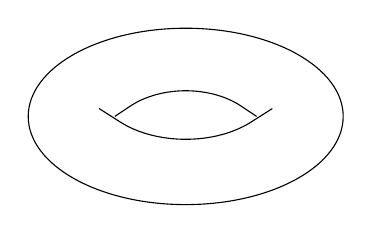
\begin{tikzpicture}
      \draw (0,0) ellipse (2 and 1.12);
      \path[rounded corners=24pt] (-.9,0)--(0,.6)--(.9,0) (-.9,0)--(0,-.56)--(.9,0);
      \draw[rounded corners=28pt] (-1.1,.1)--(0,-.6)--(1.1,.1);
      \draw[rounded corners=24pt] (-.9,0)--(0,.6)--(.9,0);
    \end{tikzpicture}
  \end{center}
  Up to continuous deformation of loops, we see that there are two non-trivial ``single'' loops in the torus, given by the red and blue loops:
  \begin{center}
    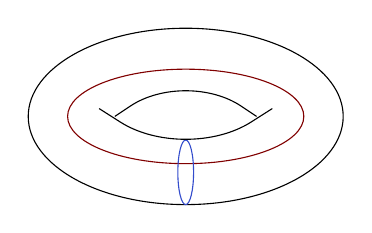
\begin{tikzpicture}
      \draw (0,0) ellipse (2 and 1.12);
      \draw [mred] (0,0) ellipse (1.5 and 0.6);

      \draw [mblue] (0, -0.71) ellipse (0.1 and 0.41);
      \path [rounded corners=24pt] (-.9,0)--(0,.6)--(.9,0) (-.9,0)--(0,-.56)--(.9,0);
      \draw [rounded corners=28pt] (-1.1,.1)--(0,-.6)--(1.1,.1);
      \draw [rounded corners=24pt] (-.9,0)--(0,.6)--(.9,0);
    \end{tikzpicture}
  \end{center}
  More generally, for an $n$ torus, we have $n$ such distinct loops $\Gamma_1, \cdots, \Gamma_n$. More concretely, after identifying $M_\mathbf{c}$ with $S^n$, these are the loops given by
  \[
    \{0\} \times \cdots \times \{0\} \times S^1 \times \{0\} \times \cdots \times \{0\} \subseteq S^1.
  \]
  We now attempt to define:
  \[
    I_j = \frac{1}{2\pi} \oint_{\Gamma_j} \mathbf{p}\cdot \d \mathbf{q},
  \]
  This is just like the formula we had for the simple harmonic oscillator.% Homologically, these are given by generators of the $1$-cycles in $H_1((M_\mathbf{c})$.

  We want to make sure this is well-defined --- recall that $\Gamma_i$ actually represents a \emph{class} of loops identified under continuous deformation. What if we picked a different loop?

  % insert picture.

  On $M_\mathbf{c}$, we have the equation
  \[
    f_i(\mathbf{q}, \mathbf{p}) = \mathbf{c}_i.
  \]
  We assume that we can invert this equation for $\mathbf{p}$ locally, ie. write
  \[
    \mathbf{p} = \mathbf{p}(\mathbf{q}, \mathbf{c}).
  \]
  The condition for being able to do so is just
  \[
    \det\left(\frac{\partial f_i}{\partial p_j}\right) \not= 0,
  \]
  which is not hard.

  Then by definition, the following holds identically:
  \[
    f_i(\mathbf{q}, \mathbf{p}(\mathbf{q}, \mathbf{c})) = c_i.
  \]
  We an then differentiate this with respect to $q_k$ to obtain
  \[
    \frac{\partial f_i}{\partial q_k} + \frac{\partial f_i}{\partial p_\ell} \frac{\partial p_\ell}{\partial q_k} = 0
  \]
  on $M_\mathbf{c}$. Now recall that the $\{f_i\}$'s are in involution. So on $M_\mathbf{c}$, we have
  \begin{align*}
    0 &= \{f_i, f_j\} \\
    &= \frac{\partial f_i}{\partial q_k} \frac{\partial f_j}{\partial p_k} - \frac{\partial f_i}{\partial p_k} \frac{\partial f_j}{\partial q_k}\\
    &= \left(-\frac{\partial f_i}{\partial p_\ell} \frac{\partial p_\ell}{\partial q_k}\right)\frac{\partial f_j}{\partial p_k} - \frac{\partial f_i}{\partial p_k}\left(-\frac{\partial f_j}{\partial p_\ell} \frac{\partial p_\ell}{\partial q_k}\right)\\
    &= \left(-\frac{\partial f_i}{\partial p_k} \frac{\partial p_k}{\partial q_\ell}\right)\frac{\partial f_j}{\partial p_\ell} - \frac{\partial f_i}{\partial p_k}\left(-\frac{\partial f_j}{\partial p_\ell} \frac{\partial p_\ell}{\partial q_k}\right)\\
    &= \frac{\partial f_i}{\partial p_k} \left(\frac{\partial p_\ell}{\partial q_k} - \frac{\partial p_k}{\partial q_\ell}\right) \frac{\partial f_j}{\partial p_\ell}.
  \end{align*}
  Recall that the determinants of the matrices $\frac{\partial f_i}{\partial p_k}$ and $\frac{\partial f_j}{\partial p_\ell}$ are non-zero. So the middle matrix must vanish! So we have
  \[
    \frac{\partial p_\ell}{\partial q_k} - \frac{\partial p_k}{\partial q_\ell} = 0.
  \]
  Since $\ell, k$ can only be $1, 2$ in this case, the only non-trivial thing this says is
  \[
    \frac{\partial p_1}{\partial q_2} - \frac{\partial p_2}{\partial q_1} = 0.
  \]
  Now suppose we have two loops $\Gamma_2$ and $\Gamma_2'$.
  % insert picture of \Gamma_2 and \Gamma_2' and surface A between them.
  Then we have
  \begin{align*}
    \left(\oint_{\Gamma_2} - \oint_{\gamma_2'}\right) \mathbf{p}\cdot \d \mathbf{q} &= \oint_{\partial A}\mathbf{p}\cdot \d \mathbf{q}\\
    &= \iint_A \left(\frac{\partial p_2}{\partial q_1} - \frac{\partial p_1}{\partial q_2}\right) \;\d q_1\;\d q_2\\
    &= 0
  \end{align*}
  by Green's theorem.

  So $I_j$ is well-defined, and
  \[
    \mathbf{I} = \mathbf{I}(\mathbf{c})
  \]
  is just a function of $c$.

  We will assume that we can invert this, so
  \[
    \mathbf{c} = \mathbf{c}(\mathbf{I}).
  \]
  We are now going to parametrize each $M_\mathbf{c}$. We are going to do so via generating functions.

  We arbitrarily pick a point $\mathbf{x}_0$, and define the generating function
  \[
    S(\mathbf{q}, \mathbf{I}) = \int_{\mathbf{x}_0}^\mathbf{x} \mathbf{p}(\mathbf{q}', \mathbf{c}(\mathbf{I})) \cdot \d \mathbf{q}',
  \]
  where $\mathbf{x} = (\mathbf{q}, \mathbf{p})$. This is just a function of $\mathbf{q}$ (and thus $\mathbf{x}$), and $\mathbf{I}$. However, this is not well-defined, because we haven't said how we are going to integrate from $\mathbf{x}_0$ to $\mathbf{x}$. We are going to pick paths arbitrarily, but we want to make sure it is well-defined. Suppose we change from a path $\gamma_1$ to $\gamma_2$ by a little bit, and they enclose a boundary $B$.

  % insert picture

  Then we have
  \[
    S(\mathbf{q}, \mathbf{I}) \mapsto S(\mathbf{q}, \mathbf{I}) + \oint_{\partial B} \mathbf{p} \cdot \d \mathbf{q}.
  \]
  Again, we are integrating $\mathbf{p} \cdot \d\mathbf{q}$ around a boundary, so there is no change.

  But what if we do something crazy, like

  % insert picture

  Then what we have effectively got is that we added a loop $\Gamma_2$ to our path, and this contributes a factor of $2\pi I_j$. So we have
  \[
    S(\mathbf{q}, \mathbf{I}) \mapsto S(\mathbf{q}, I) + 2\pi I_j.
  \]
  This is the only thing that can happen. So differentiating with repsect to $I$, we know that
  \[
    \frac{\partial S}{\partial \mathbf{I}}
  \]
  is well-defined modulo $2\pi$. These are the \emph{angles}
  \[
    \boldsymbol\phi = \frac{\partial S}{\partial \mathbf{I}}.
  \]
  Now also note that
  \[
    \frac{\partial S}{\partial \mathbf{q}} = \mathbf{p}.
  \]
  Indeed, we can write
  \[
    S = \int_{\mathbf{x}_0}^\mathbf{x} \mathbf{F} \cdot \d \mathbf{x}',
  \]
  where
  \[
    \mathbf{F} = (\mathbf{p}, 0).
  \]
  So we have
  \[
    \frac{\partial S}{\partial \mathbf{x}} = \mathbf{F},
  \]
  so
  \[
    \frac{\partial S}{\partial \mathbf{q}} = \mathbf{p}.
  \]
  In summary, we have constructed on $M_\mathbf{c}$ the following: $\mathbf{I}= \mathbf{I}(\mathbf{c})$, $S(\mathbf{q}, I)$, and
  \[
    \boldsymbol\phi = \frac{\partial S}{\partial \mathbf{I}},\quad \mathbf{p} = \frac{\partial S}{\partial \mathbf{q}}.
  \]
  So $S$ is a generator for the canonical transformation, and $(\mathbf{q}, \mathbf{p}) \mapsto (\boldsymbol\phi, \mathbf{I})$ is a canonical transformation.

  Note that at any point $\mathbf{x}$, we know $\mathbf{c} = \mathbf{f}(\mathbf{x})$. So $I(\mathbf{c}) = I(\mathbf{f})$ depends on the first integrals only. So we have
  \[
    \dot{\mathbf{I}} = 0.
  \]
  So Hamilton's equations become
  \[
    \dot{\boldsymbol\phi} = \frac{\partial \tilde{H}}{\partial \mathbf{I}},\quad \dot{\mathbf{I}} = 0 = \frac{\partial \tilde{H}}{\partial \boldsymbol\phi}.
  \]
  So the new Hamiltonian depends only on $\mathbf{I}$. So we can integrate up and get
  \[
    \boldsymbol\phi(t) = \boldsymbol\phi_0 + \Omega t,\quad \mathbf{I}(t) = I_0,
  \]
  where
  \[
    \Omega = \frac{\partial\tilde{H}}{\partial I}(I_0).
  \]
\end{proof}
To summarize, to integrate up an integrable Hamiltonian system, we identify the different cycles $\Gamma_1, \cdots, \Gamma_n$ on $M_\mathbf{c}$. We then construct
\[
  I_j = \frac{1}{2\pi} \oint_{\Gamma_j} \mathbf{p}\cdot \d \mathbf{q},
\]
where $\mathbf{p} = \mathbf{p}(\mathbf{q}, \mathbf{c})$. We then invert this to say
\[
  \mathbf{c} = \mathbf{c}(\mathbf{I}).
\]
We then compute
\[
  \boldsymbol\phi = \frac{\partial S}{\partial I_j},
\]
where
\[
  S = \int_{\mathbf{x}_0}^{\mathbf{x}} \mathbf{p}(\mathbf{q}', \mathbf{c}(\mathbf{I})) \cdot \d \mathbf{q}'.
\]
Now we do this with the Harmonic oscillator.
\begin{eg}
  In the harmonic oscillator, we have
  \[
    H(q, p) = \frac{1}{2}p^2 + \frac{1}{2}\omega^2 q^2.
  \]
  We then have
  \[
    M_\mathbf{c} = \left\{(q, p): \frac{1}{2} p^2 + \frac{1}{2}\omega^2 q^2 = c\right\}.
  \]
  The first part of the Arnold-Liouville theorem says this is diffeomorphic to $T^1 = S^1$, which it is! The next step is to pick a loop, and there is an obvious one --- the circle itself. We write
  \[
    p = p(q, c) = \pm \sqrt{2c - \omega^2 q^2}
  \]
  on $M_\mathbf{c}$. Then we have
  \[
    I = \frac{1}{2\pi} \int p \cdot \d q = \frac{c}{\omega}.
  \]
  We can then write $c$ as a function of $I$ by
  \[
    c = c(I) = \omega I.
  \]
  Now construct
  \[
    S(q, I) = \int_{x_0}^{x} p(q', c(I))\;\d q'.
  \]
  We can pick $x_0$ to be the point corresponding to $\theta = 0$. Then this is equal to
  \[
    \int_0^q \sqrt{2\omega I - \omega^2 q'^2} \;\d q'.
  \]
  To find $\phi$, we need to differentiate this thing to get
  \[
    \phi = \frac{\partial S}{\partial I} = \omega\int_0^q \frac{\d q'}{\sqrt{2 \omega I - \omega^2 q'^2}} = \sin^{-1}\left(\sqrt{\frac{\omega}{2I}}q\right)
  \]
  As expected, this is only well-defined up to a factor of $2\pi$! Using the fact that $c = H$, we have
  \[
    q = \sqrt{\frac{2\pi}{\omega}} \sin \phi,\quad p = \sqrt{2I\omega} \cos \phi.
  \]
  These are exactly the coordinates we obtained through divine inspiration last time.
\end{eg}
\section{Integrability of PDE's}
We are now going to look at PDE's. We can view these as infinite-dimensional analogues of ODE's. So what do we expect for integrable PDE's? Recall that If an $2n$-dimensional ODE is integrable, then we $n$ first integrals. Since PDE's are infinite-dimensional, and half of infinity is still infinite, we would expect to have infinitely many first integrals.

Similar to the case of integrable ODE's, we would also expect that there will be exact solutions, and we can solve general initial value problems.

Before we delve into the formal theory, we will first look at some examples of integrable PDE's, without knowing what integrable means.

\subsection{KdV equation}
\begin{eg}
  Consider the linear PDE
  \[
    u_t + u_{xxx} = 0,
  \]
  where $u = u(x, t)$ is a function on two variables. This admits solutions of the form
  \[
    e^{ikx - i\omega t},
  \]
  known as \term{plane wave modes}, so long as $\omega$ obeys the \term{dispersion relation}
  \[
    \omega = \omega(k) = -k^3.
  \]
  Thus, for \emph{any} $k$, as long as we pick $\omega$ this way, we obtain a solution. By writing the solution as
  \[
    u(x, t) = \exp\left(ik\left(x - \frac{\omega(k)}{k}t\right)\right),
  \]
  we see that plane wave modes travel at speed
  \[
    \frac{\omega}{k} = -k^2.
  \]
  It is very important that the speed depends on $k$. Different plane wave modes travel at different speeds. This is going to give rise to what we call dispersion.

  A general solution is a superposition of plane wave modes
  \[
    \sum_k a(k) e^{ikx - i \omega(k) t},
  \]
  or even an uncountable superposition
  \[
    \int_k A(k) e^{ikx - i\omega(k)t}\;\d k.
  \]
  It is a theorem that for linear PDE's on convex domains, all solutions are indeed superpositions of plane wave modes. So this is indeed completely general.

  So suppose we have an initial solution that looks like this:
  \begin{center}
    \begin{tikzpicture}[yscale=1.5]
      \draw (-2, 0) -- (2, 0);
      \draw [domain=-2:2,samples=50, mblue] plot (\x, {exp(-3 * \x * \x)});
    \end{tikzpicture}
  \end{center}
  After some time, it might look like
  \begin{center}
    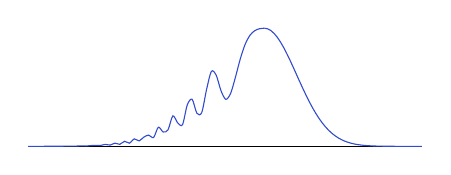
\begin{tikzpicture}[yscale=1.5]
      \draw (-3, 0) -- (2, 0);
      \draw [domain=0:2,samples=50, mblue] plot (\x, {exp(-3 * \x * \x)});
      \draw [domain=-3:0,samples=50, mblue] plot [smooth] (\x, {exp(-\x * \x) *(1 - 0.5 * sin(400*\x*\x) * sin(400*\x*\x))});
    \end{tikzpicture}
  \end{center}
  We write this as a superposition of plane wave modes. As we let time pass, different plane wave modes travel at different speeds, so this becomes a huge mess!

  Intuitively, this tells us that the third order derivative $\partial^3_x$ is what gives us dispersion.
\end{eg}

\begin{eg}
  Consider the non-linear PDE
  \[
    u_t - 6 uu_x = 0.
  \]
  This looks almost intractable, as non-linear PDE's are scary, and we don't know what to do. However, it turns out that we can solve this for any initial data $u(x, 0) = f(x)$ via the method of characteristics. The solution we get is
  \[
    u(x, t) = f(\xi),
  \]
  where $\xi$ is given implicitly by
  \[
    \xi = x - 6t f(\xi)
  \]
  We can show that $u_x$ becomes, in general, infinite in finite time. Indeed, we have
  \[
    u_x = f'(\xi) \frac{\partial \xi}{\partial x}.
  \]
  We differentiate the formula for $\xi$ to obtain
  \[
    \frac{\partial \xi}{\partial x} = 1 - 6tf'(\xi) \frac{\partial \xi}{\partial x}
  \]
  We can then check that this would indeed go to infinity in finite time, so eventually we have a straight slope. \emph{After} that, it becomes a multi-valued function! So the solution might evolve like this:

  \begin{own}
    I need some pictures.
  \end{own}
  % insert picture

  This is known as \term{wave-breaking}.

  Intuitively, we think that $-6uu_x$ corresponds to wave breaking.
\end{eg}

What happens if we combine both of these effects?
\begin{defi}[KdV equation]\index{KdV equation}
  The \emph{KdV equation} is given by
  \[
    u_t + u_{xxx} - 6 u u_x = 0.
  \]
\end{defi}
It turns out that this has a perfect balance between dispersion and non-linearity. This admits very special solutions known as \term{solitons}. For example, a $1$-solution solution is
\[
  u(x, t) = -2x^2 \sech^2 (x(x - 4xt)).
\]
The solutions tries to both topple over and disperse, and it turns out they actually move like normal. Note that the speed depends on the amplitude. So we can try to put a big one before a small one, and see what happens. It turns out they just walk pass through each other, and it seems like it is just a superposition. But the KdV solution is not linear! It does not follow the superposition principle!

These solitons are a bit like particles, and they have very little interactions with other things. They are very stable structures in the system, and that is why physicists like them a lot. We will later see that the system is in fact integrable, and we will find general $n$-soliton solutions.

\subsection{Sine-Gordon equation}

\begin{defi}[Sine-Gordon equation]\index{sine-Gordon equation}
  The \emph{sine-Gordon equation} is given by
  \[
    u_{tt} - u_{xx} + \sin u = 0.
  \]
\end{defi}
This is known as the sine-Gordon equation, because there is a famous equation in physics known as the \emph{Klein-Gordon equation}, given by
\[
  u_{tt} - u_{xx} + u = 0.
\]
Since we have a sine instead of a $u$, we call it a sine-Gordon equation!

Now let's try to motivate the equation.

Consider pendulums of length $\ell$, masses $m$ on a very long spring
\begin{center}
  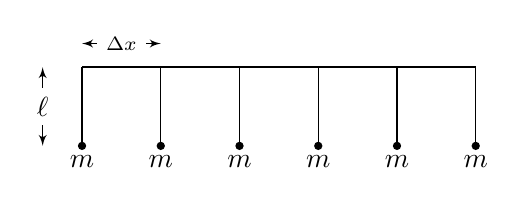
\begin{tikzpicture}
    \draw [thick] (0, 0) -- (5, 0);
    \foreach \x in {0,1,2,3,4,5} {
      \draw (\x, 0) -- (\x, -1) node [circ] {} node [below] {$m$};
    }
    \draw [latex'-latex'] (0, 0.3) -- (1, 0.3) node [pos=0.5, fill=white] {\scriptsize$\Delta x$};

    \draw [latex'-latex'] (-0.5, 0) -- (-0.5, -1) node [pos=0.5, fill=white] {$\ell$};
  \end{tikzpicture}
\end{center}
We set the pendulum in motion, and let the angle of the $i$th pendulum be $\theta_i(t) = \theta(i \Delta x, t)$ for $i \in \Z$. The gravity gives a torque of
\[
  -m\ell g \sin \theta_i.
\]
We would also expect a torque from neighbouring pendulums of magnitude, say,
\[
  \frac{K(\theta_{i + 1} - \theta_i)}{\Delta x},\quad \frac{K(\theta_{i - 1} - \theta_i)}{\Delta x}.
\]
(it doesn't really matter. We don't really care about pendulums)

By Newton's laws, we get
\[
  m\ell^2 \frac{\d^2 \theta_i}{\d t^2} = -mg \ell \sin \theta_i + \frac{K(\theta_{i + 1} - 2 \theta_i + \theta_{i - 1})}{\Delta x}.
\]
We divide everything by $\Delta x$, and take the limit as $\Delta x \to 0$, with $M = \frac{m}{\Delta x}$ held constant. We then end up with
\[
  M \ell^2 \frac{\partial^2 \theta}{\partial t^2} = - Mg\ell \sin \theta + K \frac{\partial^2 \theta}{\partial x^2}.
\]
Making some simple coordinate scaling, this becomes
\[
  u_{tt} - u_{xx} + \sin u = 0.
\]
There is also another motivation for this from differential geometry. It turns out solutions to the sine-Gordon equation correspond to pseudospherical surfaces in $\R^3$, namely the surfaces that have constant zero curvature.

If we pick ``light cone coordinates'' $\xi = \frac{1}{2}(x - t)$ and $\tau = \frac{1}{2}(x + t)$, then the sine-Gordon equations become
\[
  \frac{\partial^2}{\partial \xi \partial\tau}u = \sin u.
\]
This also admits solitons solutions
\[
  u(x, t) = 4 \tan^{-1} \left(\exp\left(\frac{x - vt}{\sqrt{1 - v^2}}\right)\right).
\]
We can check that this is indeed a solution for this non-linear PDE.

It turns out these solutions look like
\begin{center}
  \begin{tikzpicture}[xscale=0.5]
    \draw [->] (-8, 0) -- (8, 0);
    \draw [->] (-4, -0.5) -- (-4, 3);
    \draw [thick, blue] (0, 0) -- (0.01, 0);
    \draw [domain=-8:8, thick, blue] plot [smooth] (\x, {atan (exp (\x)) / 45});

    \draw [dashed] (-8, 2) -- +(16, 0);
    \node [anchor = north east] at (-4, 2) {$2\pi$};
  \end{tikzpicture}
\end{center}
Now remember that $\theta$ was an angle. So $2\pi$ is just the same as $0$! If we think of $u$ as living in $S^1$, then this satisfies the boundary condition $u \to 0$ as $x \to \pm \infty$, and we also know that no matter how this evolves, we will never get rid of this ``loop''. So the soliton is stable.

\subsection{\texorpdfstring{B\"acklund}{Backlund} transformations}
In linear partial differential equations, we have the principle of superposition --- if we have two solutions, then we can add them to get a third solution. This is no longer true in non-linear PDE's, and we don't know what to do. So we need to come up with some clever tricks to find solutions.

One solution is the \emph{B\"acklund transformation}, which originally came from geometry, where we wanted to transform a surface to another, but we will only consider the applications to PDE's.

The actual definition of the B\"acklund transformation is complicated. So we start with an example.
\begin{eg}
  Consider the Cauchy-Riemann equation
  \[
    u_x = v_u,\quad u_y = -v_x.
  \]
  If $u, v$ satisfy the Cauchy-Riemann equations, then $u, v$ are harmonic, ie. $u_{xx} + u_{yy} = 0$ etc. Suppose we already know $v = v(x, y)$ is harmonic. Then solving the Cauchy-Riemann equations gives \emph{another} harmonic function $u = u(x, y)$.

  For example, if $v = 2xy$, then we get the partial differential equations
  \[
    u_x = 2x,\quad u_y = -2y.
  \]
  So we obtain
  \[
    u(x, y) = x^2 - y^2 + C
  \]
  for some constant $C$, and this function $u$ is guaranteed to be a solution to Laplace's equations.

  So the Cauchy-Riemann equation generates new solutions to Laplace's equation from old ones. This is an example of an (auto-)B\"acklund transformation for Laplace's equation.
\end{eg}

In general, we have the following definition:
\begin{defi}[B\"acklund transformation]\index{B\"acklund transformation}
  A \emph{B\"acklund transformation} is a system of equations that relate the solutions of some PDE's to
  \begin{enumerate}
    \item A solution to some other PDE; or
    \item Another solution to the same PDE.
  \end{enumerate}
  In the second case, we call it an \term{auto-B\"acklund transformation}.
\end{defi}

Of course, the case of the Cauchy-Riemann equation is not too exciting. However, we have the following:
\begin{eg}
  Consider
  \begin{align*}
    \frac{\partial}{\partial \xi}(\varphi_1 - \varphi_2) &= 2 \varepsilon \sin \left(\frac{\varphi_1 + \varphi_2}{2}\right)\\
    \frac{\partial}{\partial \tau}(\varphi_1 + \varphi_2) &= \frac{2}{\varepsilon} \sin\left(\frac{\varphi_1 - \varphi_2}{2}\right).
  \end{align*}
  These equations come from geometry, and we will not go into details motivating these.

  We now look at the equation
  \begin{align*}
    \frac{\partial^2}{\partial \xi\partial \tau} (\varphi_1 - \varphi_2) &= \frac{\partial}{\partial \tau}\left(2\varepsilon \sin \left(\frac{\varphi_1 + \varphi_2}{2}\right)\right)\\
    &= 2\varepsilon \cos \left(\frac{\varphi_1 + \varphi_2}{2}\right)\frac{\partial}{\partial \tau}\left(\frac{\varphi_1 + \varphi_2}{2}\right)\\
    &= 2 \varepsilon \cos \left(\frac{\varphi_1 + \varphi_2}{2}\right) \frac{1}{2} \cdot \frac{2}{\varepsilon} \sin \left(\frac{\varphi_1 - \varphi_2}{2}\right)\\
    &= 2 \cos \left(\frac{\varphi_1 + \varphi_2}{2}\right)\sin \left(\frac{\varphi_1 - \varphi_2}{2}\right)\\
    &= \sin \varphi_1 - \sin \varphi_2.
  \end{align*}
  Now if $\varphi_1$ solves the sine-Gordon equations, then we have
  \[
    \frac{\partial^2 \varphi_1}{\partial \xi \partial \tau} = \sin \varphi_1.
  \]
  Then it follows that $\varphi_2$ is \emph{also} a solution to the sine-Gordon equation. So this gives an auto-B\"acklund transformation for the sine-Gordon equation.
\end{eg}

\section{Inverse scattering transform}
The inverse scattering transform is a method that allows us to integrate up equations like the sine-Gordon equations step by step, where each step involves solving a \emph{linear} equation.

\subsection{Forward scattering problem}\index{forward scattering problem}
Throughout this section, $L$ is the Schr\"odinger operator
\[
  L = -\frac{\partial^2}{\partial x^2} + u(x),
\]
where the ``potential'' $u$ has compact support, ie. $u = 0$ for $|x|$ sufficiently large. What we actually need is just that $u$ decays quickly enough as $|x| \to \infty$, but to make our life easy, we do not figure out the precise conditions to make things work, and just assume that $u$ actually vanishes for large $|x|$. We are interested in an eigenvalue (or ``spectral'') problem, ie. we want to find solutions to
\[
  L \psi = \lambda \psi.
\]
This is a ``forward'' problem, ie. given a $u$, we want to find solutions. The \emph{inverse} problem is given some sort of solutions like this, we want to find out what $u$ is.
\subsubsection{Continuous spectrum}\label{sssec:continuous-spectrum}
Here we consider solutions to $L\psi = k^2 \psi$. Since $u = 0$ for $|x|$ large, we must have
\[
  \psi_{xx} + k^2 \psi = 0
\]
for large $|x|$.

So solutions as $|x| \to \infty$ are linear combinations of $e^{\pm i k x}$. We look for specific solutions for $\psi = \varphi(x, k)$ defined by the condition
\[
  \varphi = e^{-ikx}\text{ as } x \to -\infty.
\]
Then there must be coefficients $a = a(k)$ and $b = b(k)$ such that
\[
  \phi(x, k) = a(k) e^{-ikx} + b(k) e^{ikx}\text{ as }x \to +\infty.
\]
Now, we define
\[
  \Phi(x, k) = \frac{\varphi(x, k)}{a},\quad R(k) = \frac{b(k)}{a(k)},\quad T(k) = \frac{1}{a(k)}.
\]
Here $R(k)$ is called the ``reflection'' coefficient\index{reflection coefficient}, and $A(k)$ is the ``transmission'' coefficient\index{transmission coefficient}. You may have seen these terms from IB Quantum Mechanics. We can write
\[
  \Phi(x, k) =
  \begin{cases}
    T(k) e^{-ikx} & x \to -\infty\\
    e^{-ikx} + R(k) e^{kx} & x \to +\infty
  \end{cases}.
\]
We can view the $e^{-ikx}$ term as waves travelling to the left, and $e^{ikx}$ as waves travelling to the right. When we have an incident $e^{-ikx}$ wave coming from the right, the potential reflects some portion of the wave namely $R(k) e^{ikx}$, and transmits the remaining $T(k)$. It will be shown on the first example sheet that $|T(k)|^2 + |R(k)|^2 = 1$.

What would happen when we change $k$? Since $k$ is the ``frequency'' of the wave, which is proportional to the energy we would expect that the larger $k$ is, the more of the wave is transmitted. Thus we might expect that $T(k) \to 1$, and $R(k) \to 0$. This is indeed true.

However, even if we have this, it isn't good enough. We don't just want to know what $\Phi$ looks like for large $x$. We want to know its value \emph{everywhere}.

We consider the integral equation for $f = f(x, k)$ given by
\[
  f(x, k) = f_0(x, k) + \int_{-\infty}^\infty G(x - y, k) u(y) f(y, k) \;\d y,
\]
where $f_0$ is any solution to $(\partial^2_x + k^2) f_0 = 0$, and $G$ is the Green's function $\partial^2_x + k^2$, ie. we have
\[
  (\partial_x^2 + k^2) G = \delta(x).
\]
What we want to show is that if we can find an $f$ that satisfies this integral equation, then it also satisfies the eigenvalue equation. We simply compute
\begin{align*}
  (\partial_x^2 + k^2) f &= (\partial_x^2 + k^2)f_0 + \int_{-\infty}^\infty (\partial_x^2 + k^2) G(x - y, k) u(y) f(y, k) \;\d y\\\
  &= 0 + \int_{-\infty}^\infty \delta(x - y) u(y) f(y, k)\;\d y\\
  &= u(x) f(x, k).
\end{align*}
In other words, we have
\[
  Lf = k^2 f.
\]
So it remains to prove that solutions to the integral equation exists.

This happens all of the time in mathematics. Differential equations are bad. If we differentiate a function, it might no longer be differentiable. So our operators map our functions out of the relevant function space. Integration makes functions \emph{better}. The more times we integrate, the smoother it becomes. So integral equations are always better than differential equations from a mathematical point of view.

We pick $f_0 = e^{-ikx}$ and
\[
  G(x, k) =
  \begin{cases}
    0 & x < 0\\
    \frac{1}{k} \sin (kx) & x \geq 0
  \end{cases}.
\]
Then our integral equation implies
\[
  f(x, k) = e^{-ikx}
\]
as $x \to-\infty$.

To solve the integral equation, we write this in abstract form
\[
  (I - K) f = f_0,
\]
where $I$ is the identity, and
\[
  (Kf)(x) = \int_{-\infty}^\infty G(x - y, k) u(y) f(y, k) \;\d y.
\]
So we can ``invert''
\[
  f = (I - K)^{-1} f_0.
\]
We can ``guess'' a solution to the inverse. If we don't care about rigour and just expand this, we get
\[
  f = (I + K + K^2 + \cdots)f_0.
\]
The first question to ask is if this question converges. On the second example sheet, we will show that this thing actually converges. So if this holds, then we have
\[
  (I - K)f = If_0 + K f_0 + K^2 f_0 + \cdots - (K + K^2 f_0 + K^3 f_0 + \cdots) = f_0.
\]
So this is a solution!

While we might have troubles actually evaluating this infinite sum, we can actually write the solution down in an infinite series explicitly. So the forward problem is ``trivial''.

What is the inverse problem? Suppose someone came and told us there is some potential that gives
\[
  T(k) = \frac{k}{k - i},\quad R(k) = \frac{i}{k - i}.
\]
Can we figure out what $u$ is? The answer is yes!

In fact, our brain does that all the time. When we look at things, the photons we see tell us about what photons are reflected by the wall, and our brain reconstructs the potential $u$ based on which photons are reflected, and then reconstructs $u$ and decides there is a wall! In fact, all we need to know is $R$ itself, and we can determine everything else.

This is old theory, and not too exciting. The real exciting thing is that if we have an equation
\[
  u_t + u_{xxx} - 6uu_x = 0,
\]
then we view this as a potential evolving over time, and have a starting potential $u(x, 0) = u_0(x)$. We then compute the scattering data $T$ and $R$, and then obtain the corresponding equations of evolution of the scattering data $T$ and $R$. It turns out the equations give us
\begin{align*}
  R(k, t) &= e^{8ik^3 t}R(k, 0)\\
  T(k, t) &= T(k, 0).
\end{align*}
After solving for these, we compute the inverse scattering transform to obtain $u$!

\subsection{Discrete spacetime and bound states}
So now suppose $\lambda = - \kappa^2 < 0$, where we wlog $\lambda > 0$. We are going to seek solutions to
\[
  L \psi_\kappa = - \kappa^2 \psi_\kappa.
\]
We are going to ask that
\[
  \|\psi_\lambda\|^2 = \int_{-\infty}^\infty \psi_\kappa(x)^2 \;\d x = 1.
\]
We will wlog $\psi_\kappa \in \R$. We will call these things \term{bound states}.

Since $u$ has compact support, any solution
\[
  L \varphi = - \kappa^2 \varphi
\]
must obey
\[
  \varphi_{xx} - \kappa^2 \phi = 0
\]
for $|x| \to \infty$. Then the solutions are linear combinations of $e^{\pm \kappa x}$ as $|x| \to \infty$. We now fix $\varphi_\kappa$, defined by
\[
  \varphi_\kappa(x) = e^{-\kappa x} \text{ as } x \to +\infty
\]
Then as $x \to -\infty$, there must exist coefficients $\alpha = \alpha(\kappa), \beta = \beta(\kappa)$ such that
\[
  \varphi_\kappa(x) = \alpha(\kappa) e^{\kappa x} + \beta(\kappa) e^{-\kappa x}\text{ as }x \to -\infty.
\]
We now impose the condition that $\|\psi_\kappa\|^2 = 1$, and in particular is finite. So we must have $\beta(\kappa) = 0$. It can be shown that the function $\beta = \beta(\kappa)$ has only finitely many zeroes
\[
  \chi_1 > \chi_2 > \cdots > \chi_N > 0.
\]
To show this, we will have to find out an explicit expression for the solution of $\varphi_\kappa$, just as we did for the continuous spectrum, and then explicitly find a formula of $\beta$. We can then find that it has finitely many zeros.

We now defined bound-states $\{\psi_n\}_{n= 1}^N$ by
\[
  \psi_n(x) = c_n \varphi_{\chi_{n - 1}}(x),
\]
where $c_n$ are normalization constants chosen so that $\|\psi_n\| = 1$.

\subsection{Summary of forward scattering problem}
For the spectral problem
\[
  L\psi = \lambda \psi,
\]
where
\[
  L = -\frac{\partial^2}{\partial x^2} + u,
\]
where $u$ has compact support.

In the continuous spectrum, we have $\lambda = k^2 > 0$. Then we can find some $T(k)$ and $R(k)$ such that
\[
  \Phi(x, k) =
  \begin{cases}
    T(k) e^{-ikx} & x \to -\infty\\
    e^{-ikx} + R(k) e^{kx} & x \to +\infty
  \end{cases}.
\]
In the discrete spectrum, we have $\lambda = - \kappa^2 < 0$. We can construct \emph{bound states} $\{\psi_n\}_{n = 1}^N$ such that $L\psi_n = - \chi_n^2 \psi_n$ with
\[
  \chi_1 > \chi_2 > \cdots > \chi_N > 0,
\]
and $\|\psi_n\| = 1$.

Bound states are characterized by large, positive $x$ behaviour
\[
  \psi_n(x) = c_n e^{-\chi_n x}\text{ as }x \to +\infty,
\]
where $\{c_n\}_{n = 1}^N$ are normalization constants.

Putting all these together, the scattering data for $L$ is
\[
  S = \left\{\{\chi_n, c_n\}_{n = 1}^N, R(k), T(k)\right\}.
\]
\begin{eg}
  Consider the Dirac potential $u(x) = - 2 \alpha \delta(x)$, where $\alpha > 0$. Let's try to compute the scattering data.

  We do the continuous spectrum first. Since $u(x) = 0$ for $x \not= 0$, we must have
  \[
    \Phi(x, k) =
    \begin{cases}
      T(k) e^{-ikx} & x < 0\\
      e^{-ikx} + R(k) e^{ikx} & x > 0
    \end{cases}
  \]
  Also, we want $\Phi(x, k)$ to be continuous at $x = 0$. So we must have
  \[
    T(k) = 1 + R(k).
  \]
  By integrating $L\Phi = k^2 \Phi$ over $(-\varepsilon, \varepsilon)$, taking $\varepsilon \to 0$, we find that $\frac{\partial \Phi}{\partial x}$ has a jump discontinuity at $x = 0$ given by
  \[
    ik(R - 1) + ikT = -2 \alpha T.
  \]
  We now have two equations and two unknowns, and we can solve to obtain
  \[
    R(k) = \frac{i\alpha}{k - i\alpha},\quad T(k) = \frac{k}{k - i \alpha}.
  \]
  So we have
  \[
    |R|^2 + |T|^2 = 1.
  \]
  Note that as $k$ increases, we find that $R(k) \to 0$ and $T(k) \to 1$. This makes sense, since we can think of $k$ as the energy of the wave, and the larger the energy, the more likely we are to pass through.

  Now let's do the discrete part of the spectrum, and we jump through the same hoops. Since $\delta(x) = 0$ for $x \not= 0$, we must have
  \[
    -\frac{\partial^2 \psi_n}{\partial x^2} + \chi_n^2 \psi_n = 0
  \]
  for $x \not= 0$. So we have
  \[
    \psi_n(x) = c_n e^{- \chi_n |x|}.
  \]
  Integrating $L\psi_n = - \chi_n^2 \psi_n$ over $(-\varepsilon, \varepsilon)$, we similarly find that
  \[
    c_n \chi_n = c_n \alpha.
  \]
  So there is just one bound state, with $\chi_1 = \alpha$. We finally find $c_n$ by requiring $\norm{\psi_1} = 1$. We have
  \[
    1 = \int_{-\infty}^\infty \psi_1(x)^2 \;\d x = c_1^2 \int_{-\infty}^\infty e^{-2 \chi_1|x|}\;\d x = \frac{c_1^2}{\alpha}.
  \]
  So we have
  \[
    c_1 = \sqrt{\alpha}.
  \]
  In summary, we have the following scattering data:
  \[
    S = \left\{\{\alpha, \sqrt{\alpha}\}, \frac{i\alpha}{k - i \alpha},\quad \frac{k}{k - i\alpha}\right\}.
  \]
\end{eg}
\subsection{Inverse scattering problem}
It is natural to ask: given scattering data
\[
  S = \left\{\{\chi_n, c_n\}_{n = 1}^N, R(k), T(k)\right\},
\]
can we reconstruct the potential $u = u(x)$ such that
\[
  L = -\frac{\partial^2}{\partial x^2} + u(x)
\]
has scattering data $S$? The answer is yes! Moreover, it turns out that $T(k)$ is not needed.

\begin{thm}[GLM inverse scattering theorem]\index{GLM inverse scattering theorem}
  A potential $u = u(x)$ that decays rapidly to $0$ as $|x| \to \infty$ is completely determined by its scattering data
  \[
    S = \left\{\{\chi_n, c_n\}_{n = 1}^N, R(k)\right\}.
  \]
  Given such a scattering data, if we set
  \[
    F(x) = \sum_{n = 1}^N c_n^2 e^{-\chi_n x} + \frac{1}{2\pi} \int_{-\infty}^\infty e^{ikx} R(k) \;\d k,
  \]
  and define $k(x, y)$ to be the \emph{unique} solution to
  \[
    k(x, y) + F(x + y) + \int_{x}^\infty k(x, z) f(z + y) \;\d z = 0,
  \]
  then
  \[
    u(x) = -2 \frac{\d}{\d x} k(x, x).
  \]
\end{thm}

\begin{proof}
  Too hard.
\end{proof}
Note that this equation
\[
  k(x, y) + F(x + y) + \int_{x}^\infty k(x, z) f(z + y) \;\d z = 0
\]
is not too hard to solve. We can view it as a linear equation of the form
\[
  \mathbf{x} + \mathbf{b} +A \mathbf{x} = 0
\]
for some linear operator $A$, then use our familiar linear algebra techniques to guess a solution. We can then verify that it works.

Now that we've got this result, we understand how scattering problems work. We know how to go forwards \emph{and} backwards.

\subsection{Lax pairs}
\begin{defi}[Lax pair]\index{Lax pair}
  Consider a self-adjoint linear operator
  \[
    K = a_m (x, t) \frac{\partial^m}{\partial x^m} + \cdots + a_1 (x, t) \frac{\partial}{\partial x} + a_0(x, t),
  \]
  where the $\{a_i\}$ (possibly matrix-valued) functions of $(x, t)$. If there is a second operator $A$ such that
  \[
    L_t = LA - AL = [L, A],
  \]
  where
  \[
    L_t = \dot{a}_m \frac{\partial^m}{\partial x^m} + \cdots + \dot{a}_0,
  \]
  denotes the derivative of $L$ with respect to $t$, then we call $(L, A)$ a \emph{Lax pair}.
\end{defi}

We will soon see that the existence of a Lax pair is what allows all the magic of the inverse scattering transform to work.

\begin{thm}[Isospectral flow theorem]\index{isospectral flow theorem}
  Let $(L, A)$ be a Lax pair. Then the discrete eigenvalues of $L$ are $t$-independent. Also, if $L\psi = \lambda \psi$, where $\lambda$ is a discrete eigenvalue, then
  \[
    L \tilde{\psi} = \lambda \tilde{\psi},
  \]
  where
  \[
    \tilde{\psi} = \psi_t + A \psi.
  \]
\end{thm}
The word ``isospectral'' means that we have an evolving system, but the eigenvalues are time-independent.

\begin{proof}
  Suppose we have solved the eigenvalue problem and found some
  \[
    L \psi = \lambda \psi,
  \]
  where $\lambda$ may depend on time. Then (after some rearranging) we get
  \begin{align*}
    \lambda_t \psi &= L_t \psi + L \psi_t - \lambda \psi_t\\
    &= LA \psi - AL \psi + L \psi_t - \lambda \psi_t\\
    &= LA \psi - \lambda A \psi + L \psi_t - \lambda \psi_t\\
    &= (L - \lambda)(\psi_t + A \psi)
  \end{align*}
  We now take the inner product $\psi$, and use that $\|\psi\| = 1$. We then have
  \begin{align*}
    \lambda_t &= \bra \psi, \lambda_t \psi\ket\\
    &= \bra \psi, (L - \lambda)(\psi_t + A_\psi)\ket\\
    &= \bra (L - \lambda)\psi, \psi_t + A_\psi\ket\\
    &= 0,
  \end{align*}
  using the fact that $L$, hence $L - \lambda$ is self-adjoint.

  So we know that $\lambda_t = 0$, ie. that $\lambda$ is time-independent. Then our above equation gives
  \[
    L \tilde{\psi} = \lambda \tilde{\psi},
  \]
  where
  \[
    \tilde{\psi} = \psi_t + A\psi.
  \]
\end{proof}

\begin{eg}
  Consider
  \begin{align*}
    L =- \frac{\partial^2}{\partial x^2} + u(x, t)\\
    A = 4 \partial_x^3 - 3 (u \partial_x + \partial_x u).
  \end{align*}
  Then $(L, A)$ is a Lax pair iff $u = u(x, t)$ satisfies KdV. In other words, we find that
  \[
    L_t - [L, A] = 0 \Leftrightarrow u_t + u_{xxx} - 6uu_x =0 .
  \]
\end{eg}

\subsection{Evolution of scattering data}
Now we do the clever bit: we allow the potential $u = u(x, t)$ to evolve via KdV
\[
  u_t + u_{xxx} - 6 u u_x = 0.
\]
We see how the scattering data for $L = -\partial_x^2 + u(x, t)$ evolves. Again, we will assume that $u$ has compact support. Note that this implies that we have
\[
  A = 4 \partial_x^3\text{ as }|x| \to \infty.
\]
\subsubsection{Continuous spectrum (\texorpdfstring{$\lambda = k^2 > 0$}{lambda = k^2 > 0})}
As in Section \ref{sssec:continuous-spectrum}, for each $t$, we can construct a solution $\varphi$ to $L \varphi = \kappa^2 \varphi$ such that
\[
  \varphi(x, t) =
  \begin{cases}
    e^{-ikx} & x \to -\infty\\
    a(k, t) e^{-ikx} + b(k, t) e^{ikx} & x \to \infty
  \end{cases}.
\]
As with the proof of the isospectral flow theorem, we can differentiate the equation
\[
  L^2 = k^2 \varphi
\]
with $k^2 > 0$ fixed to get
\[
  0 = (L - k^2)(\varphi_t + A_\varphi).
\]
This tells us that
\[
  \tilde{\varphi} = \varphi_t + A \varphi
\]
solves
\[
  L \tilde{\varphi} = k^2 \tilde{\varphi}.
\]
We can try to figure out what $\tilde{\varphi}$ is for large $|x|$. We recall that for large $|x|$, we simply have $A = 4 \partial_x^3$. Then we can write
\[
  \tilde{\varphi}(x, t) =
  \begin{cases}
    4 ik^3 e^{-ikx} & x \to -\infty\\
    (a_t + 4 ik^3 a)e^{-ikx} + (b_t - 4ik^3 b) e^{ikx} & x \to \infty
  \end{cases}
\]
We now consider the function
\[
  \theta = 4ik^3 \varphi - \tilde{\varphi}.
\]
By linearity of $L$, we have
\[
  L \theta = k^2 \theta.
\]
Note now that by construction, we had $\theta(x, t) \to 0$ as $x \to -\infty$.

Recall that the solution to $Lf = k^2 f$ for $f = f_0$ as $x \to -\infty$ is just
\begin{align*}
  f &= (I - K)^{-1} f_0\\
  &= (I + K + K^2 + \cdots)f_0
\end{align*}
So we obtain
\[
  \theta = (1 + K + K^2 + \cdots) 0 = 0.
\]
So we must have
\[
  \tilde{\varphi} = 4ik^3 \varphi.
\]
Looking at the $x \to +\infty$ behaviour, we figure that
\begin{align*}
  a_t + 4ik^3 a &= 4 ik^3 a\\
  b_t - 4ik^3 b &= 4ik^3 b
\end{align*}
Of course, these are equations we can solve. We have
\begin{align*}
  a(k, t) &= a(k, 0)\\
  b(k, t) &= b(k, 0) e^{8ik^3 t}
\end{align*}.
In terms of the reflection and transmission coefficients, we have
\begin{align*}
  R(k, t) &= R(k, 0) e^{8ik^3 t}\\
  T(k, t) &= T(k, 0)
\end{align*}
Recall that we started with the \emph{really} complicated KdV equation. And the scattering data evolves in such a simple way. This is \emph{AMAZING}.

\subsubsection{Discrete spectrum (\texorpdfstring{$\lambda= -\kappa^2 < 0$}{lambda = -kappa^2 < 0})}
For each $t$, we can construct bound states $\{\psi_n(x, t)\}_{n = 1}^N$ such that $L\psi_n = - \chi_n^3 \psi_n$ and $\|\psi_n\| = 1$. Moreover, we have
\[
  \psi_n(x, t) = c_n(t) e^{-\chi_n|x|}.
\]
From the isospectral theorem, we know that the $\chi_n$'s are constant, and we have
\[
  \tilde{\psi}_n = \partial_t \psi_n + A\psi_n
\]
satisfies
\[
  L\tilde{\psi}_n = - \chi_n^2 \tilde{\psi}_n
\]
It is an exercise to show that these solutions must actually be proportional to one another. Looking at Wronskians, we can show that $\tilde{\psi}_n \propto \psi_n$. Also, we have
\[
  \bra \psi_n, \tilde{\psi}_n\ket = \int_{-\infty}^\infty \psi_n(x, t) \tilde{\psi}_n(x, t) \;\d x = 0.
\]
\begin{align*}
  \bra \psi_n, \tilde{\psi}_n\ket &= \bra \psi_n \partial_t \psi_n\ket + \bra\psi_n, A \psi_n\ket\\
  &= \frac{1}{2} \frac{\partial}{\partial t} \bra \psi_n, \psi_n\ket + \bra \psi_n, A \psi_n\ket
\end{align*}
using the fact that $A$ is antisymmetric and $\|\psi_n\|$ is constant. We thus deduce that $\tilde{\psi}_n = 0$.

By large $x$-behaviour, we have
\[
  \tilde{\psi}_n(x, t) = (\dot{c}_n - 4 \chi_n^3 c_n) e^{- \chi_n x}
\]
as $x \to +\infty$. Since $\tilde{\psi}_n \equiv = 0$, we must have
\[
  \dot{c}_n - 4 \chi_n^3 c_n = 0.
\]
So we have
\[
  c_n(t) = c_n(0) e^{4 \chi_n^3 t}.
\]
This is again \emph{AMAZING}.

So in summary, if $u = u(x, t)$ evolves according to KdV, namely
\[
  u_t + u_{xxx} - 6uu_x = 0,
\]
then the scattering data for $L = -\partial_x^2 + u$ is
\[
  S(t) = \left\{\{\chi_n, c_n(0)e^{4\chi_n^3 t}\}_{n = 1}^N, R(k, 0)e^{8ik^3 t}\right\}.
\]
So if we have an initial value problem, we do the forward transform problem to find the initial scattering data $S(0)$. We then do the trivial steps above to find the scattering data $S(t)$ for all time $t$. We then apply GLM to obtain $u(x, t)$ for all time $t$.
\[
  \begin{tikzcd}[row sep=5em, column sep=8em]
    u_0(x) \ar[r, "\text{Construct scattering data}", "L = -\partial_x^2 + u_0(x)"'] \ar[d, "\text{KdV equation}"] & S(0) = \left\{\{\chi_n, c_n(0)\}_{n = 1}^N, R(k, 0)\right\} \ar[d, "\text{Evolve scattering data}"', "{L_t = [L, A]}"]\\
    u(x, t) & S(t) = \left\{\{\chi_n, c_n(0)e^{4\chi_n^3 t}\}_{n = 1}^N, R(k, 0)e^{8ik^3 t}\right\} \ar[l, "\text{Solve GLM equation}"]
  \end{tikzcd}
\]
The key thing that makes this work is that $u_t + u_{xxx} - 6 uu_x$ holds if and only if $L_t = [L, A]$.

For comparison, this is what we would do if we had to solve $u_t + u_{xxx} = 0$: we take the Fourier transform:
\[
  \begin{tikzcd}[row sep=5em, column sep=8em]
    u_0(x) \ar[r, "\text{Fourier transform}"] \ar[d, "u_t + u_{xxx} = 0"] & \hat{u}_0(k) \ar[d, "\hat{u}_t - ik^3 \hat{u} = 0"]\\
    u(x, t) & \hat{u}(u, t) = \hat{u}_0(k) e^{ik^3 t} \ar[l, "\text{Inverse Fourier}"', "\text{Transform}"]
  \end{tikzcd}
\]
It is just the same steps, but with a simpler transform!

\subsection{Reflectionless potentials}
We are now going to actually solve the KdV equation for a special kind of potential --- reflectionless potential.

\begin{defi}[Reflectionless potential]\index{reflectionless potential}\index{potential!reflectionless}
  A \emph{reflectionless potential} is a potential $u(x, 0)$ if $R(k, 0) = 0$.
\end{defi}

Now if $u$ evolves according to the KdV equation, then
\[
  R(k, t) = R(k, 0) e^{8ik^3 t} = 0.
\]
So if a potential starts off reflectionless, then it remains reflectionless.

We now want to solve the GLM equation in this case. Using the notation when we wrote down the GLM equation, we simply have
\[
  F(x) = \sum_{n = 1}^N c_n^2 e^{-\chi_n x}.
\]
We will mostly not write out the $t$ when we do this, and only put it back in at the very end. We now guess that the GLM equation has a solution of the form
\[
  K(x, y) = \sum_{m = 1}^N K_m(x) e^{-\chi_m y}
\]
for some unknown functions $\{K_m\}$. We substitute this into the GLM equation and find that
\[
  \sum_{n = 1}^N \left[c_n^2 e^{-\chi_n x}+ K_n(x) + \sum_{m = 1}^N c_n^2 K_m(x) \int_x^\infty e^{-(\chi_n + \chi_m)z}\;\d z\right] e^{-\chi_n y} = 0.
\]
Now notice that the $e^{-\chi_n y}$ for $n = 1, \cdots, N$ are linearly independent. So we actually have $N$ equations, one for each $n$. So we know that
\[
  c_n^2 e^{-\chi_n x} + K_n(x) + \sum_{m = 1}^N \frac{c_n^2 K_m(x)}{\chi_n + \chi_m} e^{-(\chi_n + \chi_m)x} = 0\tag{$*$}
\]
for all $n = 1, \cdots, N$. Now if our goal is to solve the $K_n(x)$, then this is just a linear equation for each $x$!. We set
\begin{align*}
  \mathbf{c} &= (c_1^2 e^{-\chi_1 x}, \cdots, c_N^2 e^{-\chi_N x})^T\\
  \mathbf{K} &= (K_1(x), \cdots, K_N(x))^T\\
  A_{nm} &= \delta_{nm} + \frac{c_n^2 e^{-(\chi_n - \chi_m)x}}{\chi_n + \chi_m}.
\end{align*}
Then $(*)$ becomes
\[
  A\mathbf{K} = -\mathbf{c}.
\]
This really is a linear algebra problem. But we don't really have to solve this. The thing we really want to know is
\begin{align*}
  K(x, x) &= \sum_{m = 1}^N K_m(x) e^{-\chi_m x}\\
  &= \sum_{m = 1}^N \sum_{m = 1}^N (A^{-1})_{mn} (-\mathbf{c})_n e^{-\chi_m x}
\end{align*}
Now note that
\[
  \frac{\d}{\d x}A_{nm}(x) = A_{nm}'(x) = - c_n^2 e^{-\chi_n x} e^{-\chi_m x} = (-\mathbf{c})_n e^{-\chi_m x}.
\]
So we can replace the above thing by
\[
  K(x, x) = \sum_{m = 1}^N \sum_{n = 1}^N (A^{-1})_{mn} A'_{nm} = \tr(A^{-1}A').
\]
It is an exercise on the second example sheet to show that this is equal to
\[
  K(x, x) = \frac{1}{\det A} \frac{\d}{\d x} (\det A) = \frac{\d}{\d x} \log (\det A).
\]
So we have
\[
  u(x) = - 2 \frac{\d^2}{\d x^2} \log(\det A).
\]
We now put back the $t$-dependence we didn't bother to write all along. Then we have
\[
  u(x, t) = -2 \frac{\partial^2}{\partial x^2} \log(\det A(x, t)),
\]
where
\[
  A_{nm}(x, t) = \delta_{nnm} + \frac{c_n(0)^2 e^{8\chi_n^3 t}e^{-(\chi_n + \chi_m)x}}{\chi_n + \chi_m}.
\]
It turns out these are soliton solutions, and the number of discrete eigenstates $N$ is just the number of solitons!
\subsection{Infinitely many first integrals}
As we've previously mentioned, we are expecting our integrable PDE's to have infinitely many first integrals. Recall we can construct $\varphi = \varphi(x, k, t)$ such that
\[
  L\varphi = k^2 \varphi,
\]
and we had
\[
  \varphi(x, k, t) =
  \begin{cases}
    e^{-ikx} & x \to -\infty\\
    a(k, t) e^{-ikx} + b(k, t) e^{ikx} & x \to \infty
  \end{cases}.
\]
But when we looked at the evolution of the scattering data, we can actually write down what $a$ and $b$ are. In particular, $a(k, t) = a(k)$ is independent of $t$. So we might be able to extract some first integrals from it. We have
\[
  e^{ikx} \varphi(x, k, t) = a(k) + b(k, t) e^{2ikx} \text{ as }x \to \infty.
\]
We now take the average over $[R, 2R]$ for $R \to \infty$, we have
\[
  \frac{1}{R} \int_R^{2R} a(k) \;\d x = a(k).
\]
For the $b(k, t)$ term, we have
\[
  \frac{1}{R} \int_R^{2R} b(k, t) e^{2ikx} \;\d x = O\left(\frac{1}{R}\right),
\]
So we have
\begin{align*}
  a(k) &= \lim_{R \to \infty} \frac{1}{R} \int_R^{2R} e^{ikx} \varphi(x, k, t) \;\d x\\
  &= \lim_{R \to \infty} \int_1^2 e^{ikRx} \varphi(Rx, k, t) \;\d x.
\end{align*}
So can we figure out what this thing is? Since $\varphi = e^{-ikx}$ as $x \to -\infty$, it is ``reasonable'' to write
\[
  \varphi(x, k, t) = \exp\left(-ikx + \int_{-\infty}^x S(y, k, t)\;\d y\right)
\]
for some function $S$. Then after some dubious manipulations, we would get
\begin{align*}
  a(k) &= \lim_{R \to \infty} \int_1^2 \exp\left(\int_{-\infty}^{Rx} S(y, k, t)\;\d y\right)\;\d x\\
  &= \exp\left(\int_{-\infty}^\infty S(y, k, t)\;\d y\right).\tag{$\dagger$}
\end{align*}
Now this is interesting, since the left hand side $a(k)$ has no $t$-dependence, but the right-hand formula does. So this is where we get our first integrals from.

Now we need to figure out what $S$ is. To find $S$, recall that $\varphi$ satisfies
\[
  L\varphi = k^2 \varphi.
\]
So we just try to shove our formula of $\varphi$ into this equation. Notice that
\[
  \varphi_x = (S - ik) \varphi,\quad \varphi_{xx} = S_x \varphi + (S - ik)^2 \varphi.
\]
We then put these into the Schr\"odinger equation to find
\[
  S_x - (2ik)S + S^2 = -u.
\]
We have got no $\varphi$'s left. This is a famous type of equation --- a \term{Ricatti-type equation}. We can make a guess
\[
  S(x, k, t) = \sum_{n = 1}^\infty \frac{S_n(x, t)}{(2ik)^n}.
\]
This seems like a strange thing to guess, but there are indeed some good reasons for this we will not get into. Putting this into the equation and comparing coefficients of $k^{-n}$, we obtain a recurrence relation
\begin{align*}
  S_1 &= -u\\
  S_{n + 1} &= \frac{\d S_n}{x} + \sum_{m = 1}^{n - 1} S_m S_{n - m}.
\end{align*}
This is a straightforward recurrence relation to compute. We can make a computer do this, and get
\[
  S_2 = -u_x,\quad S_3 = -u_{xx} + u^2,\quad S_4 = \cdots
\]
Using the expression for $S$ in $(\dagger)$, we find that
\begin{align*}
  \log a(k) &= \int_{-\infty}^\infty S(x, k, t) \;\d t\\
  &= \int_{-\infty}^\infty \frac{1}{(2ik)^n} \int_{-\infty}^\infty S_n(x, t)\;\d x.
\end{align*}
Since the LHS is time-independent, so is the RHS. By comparing coefficients of $k$, we know that each
\[
  \int_{-\infty}^\infty S_n (x, t)\;\d t
\]
must be constant with time!

Looking at the first few terms, for $n = 1$, we find a first integral
\[
  \int_{-\infty}^\infty u(x, t)\;\d x
\]
We can view this as a conservation of mass.

For $n = 2$, we obtain a first integral
\[
  \int_{-\infty}^\infty u_x(x, t)\;\d x.
\]
This is actually boring, since we assumed that $u$ vanishes at infinity. So we knew this is always zero anyway.

For $n = 3$, we have
\[
  \int_{-\infty}^\infty (-u_{xx}(x, t) + u(x, t)^2) \;\d x = \int_{-\infty}^\infty u(x, t)^2 \;\d x.
\]
This is in some sense a conservation of momentum.

It is an exercise to show that $S_n$ is a total derivative for all even $n$, so we don't get any interesting conserved quantity.

\section{Structure of integrable PDEs}
\subsection{Infinite dimensional Hamiltonian system}
Recall that a (finite-dimensional) Hamiltonian system is governed by
\[
  \frac{\d \mathbf{x}}{\d t} = J \frac{\partial H}{\partial \mathbf{x}},
\]
where $\mathbf{x}(t)$ is a vector of length $2n$, $J$ is an anti-symmetric matrix, and $H = H(\mathbf{x})$ is the Hamiltonian. What do we do if we want to promote this to infinite-dimensional systems?

When we want to describe an infinite-dimensional system, we rarely write down a vector of infinite length. Instead, we think of it as a function $u(x, t)$ depending not only on $t$, but also some ``$x$'', where $x$ belongs to some infinite set $\Omega$. We will usually just take $\Omega = \R$.

What would be the natural generalization of a Hamiltonian system? We now see how we can generalize certain concepts from the finite-dimensional case to the infinite-dimensional phase space. These are just heuristics, and we will make proper definitions later on.
\begin{center}
  \begin{tabular}{cc}
    \toprule
    $2n$-dimensional phase space & infinite dimensional phase space\\
    \midrule
    $(\mathbf{x})_i(t): i = 1, \cdots, 2n$ & $u(x, t): x \in \Omega$\\
    $\mathbf{x}\cdot\mathbf{y} = \sum_i x_i y_i$ & $\bra u, v \ket = \int_\omega u(x, t) v(x, t) \;\d x$\\
    $\frac{\d}{\d t}$ & $\frac{\partial}{\partial t}$\\
    $\frac{\partial}{\partial \mathbf{x}}$ & ``$\frac{\delta}{\delta u}$''\\
    $J$ anti-symmetric matrix & $\mathcal{J}$ anti-symmetric linear operator\\
    $f = f(\mathbf{x})$ (functions) & $F = F[u]$ (functionals)\\
    \bottomrule
  \end{tabular}
\end{center}
Here the $\frac{\delta}{\delta u}$, is the ``functional derivative'' we've seen in variational calculus.

Now let's try to go through these things, starting with the definition of a functional:
\begin{defi}[Functional]\index{functional}
  A \emph{functional} $F$ is a real-valued function (on some function space) of the form
  \[
    F[u] = \int_\Omega f(x, u, u_x, u_{xx}, \cdots)\;\d x.
  \]
\end{defi}
Because we are lazy, we will just write $\int \d x$ for $\int_{-\infty}^\infty \d x$.

We next talk about the idea of a functional derivative.
\begin{defi}[Functional derivative/Euler-Lagrange derivative]\index{functional derivative}\index{Euler-Lagrange derivative}
  The \emph{functional derivative} of $F = F[u]$ at $u$ is the unique function $\delta F$ satisfying
  \[
    \bra \delta F, \eta\ket = \lim_{\varepsilon \to 0} \frac{F[u + \varepsilon \eta] - F[u]}{\varepsilon}
  \]
  for all smooth $\eta$ with compact support.

  Alternatively, we have
  \[
    F[u, \varepsilon \eta] = F[u] + \varepsilon \bra \delta F, \eta\ket + o (\varepsilon).
  \]
  Note that $\delta F$ is a function, depending on $u$.
\end{defi}

\begin{eg}
  Set
  \[
    F[u] = \frac{1}{2} \int u_x^s \;\d x.
  \]
  We then have
  \begin{align*}
    F[u + \varepsilon \eta] &= \frac{1}{2}\int (u_x + \varepsilon \eta_x)^2 \;\d x\\
    &= \frac{1}{2} u_x^2 \;\d x + \varepsilon \int u_x \eta_x \;\d x + o(\varepsilon)\\
    &= F[u] + \varepsilon \bra u_x, \eta_x\ket + o(\varepsilon)\\
    \intertext{This is no good, because we want something of the form $\bra \delta F, \eta\ket$, not an inner product with $\eta_x$. When in doubt, integrate by parts!}
    &= F[u] + \varepsilon \bra -u_{xx}, \eta\ket + o(\varepsilon).
  \end{align*}
  Note that when integrating by parts, we don't have to mess with the boundary terms, because $\eta$ is assumed to have compact support. So we have
  \[
    \delta F = - u_{xx}.
  \]
\end{eg}
in general, from IB Variational Principles, we know that if
\[
  F[u] = \int f(x, u, u_x, u_{xx}, \cdots)\;\d x,
\]
then we have
\[
  \delta F = \frac{\partial f}{\partial u} - \D_x\left(\frac{\partial f}{\partial u_x}\right) + \D_x^2 \left(\frac{\partial f}{\partial u_{xx}}\right) - \cdots.
\]
Here $D_x$ is the total derivative.
\begin{eg}
  We have
  \[
    \frac{\partial}{\partial x}(xu) = u,\quad \D_x (xu) = u + x u_x.
  \]
\end{eg}
Recall that for finite-dimensional Hamiltonian systems, we were able to define a Poisson bracket for $f = f(\mathbf{x}), g = g(\mathbf{x})$, given by
\[
  \{f, g\} = \frac{\partial f}{\partial \mathbf{x}} \cdot J \frac{\partial g}{\partial \mathbf{x}}.
\]
We knew that this is bilinear, antisymmetric and satisfies the Jacobi identity.

How do we promote this to infinite-dimensional Hamiltonian systems? We can just replace $\frac{\partial f}{\partial \mathbf{x}}$ with the functional derivative, the dot with the inner product, and the $J$ with our funny $\mathcal{J}$. We have not yet figured out what $\mathcal{J}$ really should be, but assuming we have found a reasonable linear and antisymmetric candidate, we can make the following definition:

\begin{defi}[Poisson bracket for infinite-dimensional Hamiltonian systems]\index{Poisson bracket!infinite-dimensional}
  We define the \emph{Poisson bracket} for two functionals to be
  \[
    \{F, G\} = \bra \delta F, \mathcal{J} \delta G\ket = \int \delta F(x) \mathcal{J} \delta G(x)\;\d x.
  \]
\end{defi}
Since $\mathcal{J}$ is linear and antisymmetric, we know that this Poisson bracket is bilinear and antisymmetric. The annoying part is the Jacobi identity
\[
  \{F, \{G, H\}\} + \{G, \{H, F\}\} + \{H, \{F, G\}\} = 0.
\]
This is \emph{not} automatically satisfied. We need conditions on $\mathcal{J}$. The simplest antisymmetric linear map we can think of would be $\mathcal{J} = \partial_x$, and this works, ie. the Jacobi identity is satisfied. Proving that is easy, but painful.

Recall that for finite-dimensional systems, our equation of evolution is given by
\[
  \frac{\d}{\d t} \mathbf{x} = J \frac{\partial H}{\partial \mathbf{x}}.
\]
We make the obvious analogues here:
\begin{defi}[Hamiltonian form]\index{Hamiltonian form}
  An evolution equation for $u = u(x, t)$ is in \emph{Hamiltonian form} if it can be written as
  \[
    u_t = \mathcal{J} \frac{\delta H}{\delta u}.
  \]
  for some functional $H = H[u]$ and some linear, antisymmetric $\mathcal{J}$ such that the Poisson bracket
  \[
    \{F, G\} = \bra \delta F, \mathcal{J} \delta G\ket
  \]
  obeys the Jacobi identity.
\end{defi}

Such a $\mathcal{J}$ is known as a Hamiltonian operator.
\begin{defi}[Hamiltonian operator]\index{Hamiltonian operator}
  A \emph{Hamiltonian operator} is linear antisymmetric function $\mathcal{J}$ on the space of functions such that the induced Poisson bracket obeys the Jacobi identity.
\end{defi}

Now a natural question to ask is when the results for finite-dimensional cases hold for infinite-dimensional cases. Often in mathematics, life is not so fortunate. Things that hold for finite-dimensional systems need not hold for infinite-dimensional cases. It turns out that for us, many do carry over, but we do not have time to cover all of them.

Note that it is possible that the same PDE might be able to be put into Hamiltonian form for \emph{different} $\mathcal{J}$'s. These are known as \emph{bihamiltonian systems}.
\begin{defi}[Bihamiltonian system]\index{bihamiltonian system}
  A PDE is \emph{bihamiltonian} if it can be written in Hamiltonian form for differen $\mathcal{J}$.
\end{defi}
It turns out that when this happens, then the system has infinitely many first integrals in involution! We will prove this later on.

We now try to derive some results we had in the finite-dimensional case. Recall that for $f = f(\mathbf{x})$, we had
\[
  \frac{\d f}{\d t} = \{f, H\}.
\]
This generalizes to the infinite-dimensional case.
\begin{prop}
  If $u_t = \mathcal{J} \delta H$ and $i = I[u]$, then
  \[
    \frac{\d I}{\d t} = \{I, H\}.
  \]
  In particular $I[u]$ is a first integral of $u_t = \mathcal{J} \delta H$ iff $\{I, H\} = 0$.
\end{prop}

\begin{proof}
  If
  \[
    I[u] = \int i(x, u, u_x, u_{xx}, \cdots)\;\d x,
  \]
  then we have
  \begin{align*}
    \frac{\d I}{\d t} &= \frac{\d}{\d t} \int i(x, u, u_x, \cdots) \;\d x\\
    &= \int \frac{\partial }{\partial t}i(x, u, u_x, \cdots)\;\d x\\
    &= \int \left(u_t \frac{\partial i}{\partial u} + u_{tx} \frac{\partial i}{\partial u_x} + u_{txx} \frac{\partial i}{\partial u_{xx}} + \cdots\right)\;\d x\\
    \intertext{These terms look horrible. We don't want $u_{tx}$ terms. We just what $u_t$. So we again integrate by parts:}
    &= \int \left(\frac{\partial i}{\partial u} - D_x\left(\frac{\partial i}{\partial u_x}\right) + \D_x^2 \left(\frac{\partial i}{\partial u_{xx}}\right) + \cdots\right)u_t \;\d x\\
    &= \int \delta I u_t \;\d x\\
    &= \bra \delta I, u_t\ket\\
    &= \bra \delta I, \mathcal{J} \delta H\ket\\
    &= \{I, H\}.
  \end{align*}
\end{proof}

One can show that the KdV equation is Hamiltonian, and each of the first integrals we found would Poisson-commute with $H$.

\subsection{KdV Hierarchy}
We are going to write down a hierarchy of KdV equations. The KdV equation can be written in Hamiltonian form
\begin{align*}
  u_t &= \mathcal{J}_1 \delta H_1,\\
  \mathcal{J} &= \frac{\partial}{\partial x},\\
  H_1[u] &=\int \frac{1}{2}u_x^2 + u^3 \;\d x.
\end{align*}
We can check that this says
\begin{align*}
  u_t &= \frac{\partial}{\partial x}\left(\frac{\partial}{\partial u} - D_x \left(\frac{\partial}{\partial u_x}\right)\right)\left(\frac{1}{2}u_x^2 + u^3\right)\\
  &= 6uu_x- u_{xxx},
\end{align*}
and this is the KdV equation.

More interestingly, we can write this in Hamiltonian form in two distinct ways. We also have
\[
  u_t = \mathcal{J}_0 \delta H_0,\quad \mathcal{J}_0 = - \frac{\partial^3}{\partial x^3} + 4u \partial_x + 2 u_x,\quad H_0[u] = \int \frac{1}{2}u^2 \;\d x.
\]
So KdV is bi-Hamiltonian. We then know that
\[
  \mathcal{J}_1 \delta H_1 = \mathcal{J}_0 \delta H_0.
\]
For ease of notation, we set $\mathcal{J}_1 = \partial_x$ and $\mathcal{J}_0 = \mathcal{J}$. We can then define a sequence of Hamiltonians $\{H_n\}_{n \geq 0}$ via
\[
  \partial_x\delta H_{n + 1} = \mathcal{J} \delta H_n.
\]
We will assume that we can always solve for $H_{n + 1}$ given $H_n$. This can be proven, but we shall not. We can then start investigating what this sequence of Hamiltonians are like.

\begin{thm}
  Let $\{H_n\}_{n \geq 0}$ and $\mathcal{J}$ be as above. Then if $u_t = \partial_x \delta H_1$, then $\{H_n\}_{n \geq 0}$ are all first integrals of KdV in involution, ie.
  \[
    \{H_n, H_n\} = 0.
  \]
\end{thm}

\begin{proof}
  We notice the following interesting fact:
  \begin{align*}
    \{H_n, H_m\} &= \bra \delta H_n, \partial_x \delta H_m\ket\\
    &= \bra \delta H_n, \mathcal{J} \delta H_{m - 1}\ket\\
    &= - \bra \mathcal{J} \delta H_n, \delta H_{m - 1}\ket\\
    &= - \bra \partial_x \delta H_{n + 1}, \delta H_{m - 1}\ket\\
    &= \bra \delta H_{n + 1}, \partial_x \delta H_{m - 1}\ket\\
    &= \{H_{n + 1}, H_{m - 1}\}.
  \end{align*}
  Iterating this many times, we find that
  \[
    \{H_n, H_m\} = \{H_m, H_n\}.
  \]
  Then by antisymmetry, they must both vanish. So done.
% We already know $H_0$ is a first integral, We want to show that
% \[
% \frac{\d}{\d t} = \{H_1, H_m\} = \bra \delta H_1, \partial_x \delta H_m\ket = 0.
% \]
% We have
\end{proof}

\subsection{Zero curvature representation}
Let $U = U(\lambda)$ and $V = V(\lambda)$ be $N \times N$ matrices that depend on $(x, t; \lambda)$. The $\lambda$ will be thought of as a ``\term{spectral parameter}'', like the $\lambda$ in the eigenvalue problem $L \varphi = \lambda \varphi$. Usually, the $U$ and $V$ will not depend on $x$ and $t$ implicitly, but will instead depend on some function $u(x, t)$ and its derivative.

Consider the PDE's
\[
  \frac{\partial}{\partial x}\mathbf{v} = U(\lambda) \mathbf{v},\quad \frac{\partial}{\partial t} \mathbf{v} = V(\lambda) \mathbf{v},\tag{$\dagger$}
\]
where $\mathbf{v} = \mathbf{v}(x, t; \lambda)$ is an $N$-dimensional vector. This is a two-way problem --- we could be given the $U, V$, and we want to find some $\mathbf{v}$ that works. On the other hand, we might also be given a $\mathbf{v}$ that works, and we want to find the $U, V$.

Now notice that here we have twice as many equations as there are unknowns. So we need some compatibility conditions. We use the fact that $\mathbf{v}_{xt} = \mathbf{v}_{tx}$. So we need
\begin{align*}
  0 &= \frac{\partial}{\partial t} U(\lambda) \mathbf{v} - \frac{\partial}{\partial x}V(\lambda) \mathbf{v}\\
  &= \frac{\partial U}{\partial t} \mathbf{v} + U \frac{\partial \mathbf{v}}{\partial t} - \frac{\partial V}{\partial x}\mathbf{v} - V \frac{\partial \mathbf{v}}{\partial x}\\
  &= \frac{\partial U}{\partial t}\mathbf{v} + UV \mathbf{x} - \frac{\partial V}{\partial x}\mathbf{v} - VU \mathbf{v}\\
  &= \left(\frac{\partial U}{\partial t} - \frac{\partial V}{\partial x} + [U, V]\right) \mathbf{v}.
\end{align*}
There is a beautiful theorem by Frobenius that if this equation holds, then there is always a solution.

If we want the equation to always have a solution for any initial $\mathbf{v}_0$, we know the above equation must hold for any $\mathbf{v}$. So we must have
\[
  \frac{\partial U}{\partial t} - \frac{\partial V}{\partial x} + [U, V] = 0
\]
These are known as the \term{zero curvature equations}.

Why are these called the zero curvature equations. In geometry, a connection $A$ on a tangent bundle has zero curvature if
\[
  \frac{\partial A_j}{\partial x_i} - \frac{\partial A_i}{\partial x_j} + [A_i, A_j] = 0.
\]
In General Relativity, we use covariant derivatives
\[
  \nabla = \partial + \Gamma.
\]
(with loads of indices everywhere which we omit) We can show that the Riemann curvature tensor is
\[
  R = \partial \Gamma - \partial \Gamma + \Gamma \Gamma - \Gamma \Gamma,
\]
where we have indices everywhere, and in particular, the terms that look the same aren't because they have indices. Then spacetime has zero curvature iff $R = 0$.

\begin{eg}
  Consider
  \[
    U(\lambda) = \frac{i}{2}
    \begin{pmatrix}
      2\lambda & u_x\\
      u_x & -2\lambda
    \end{pmatrix},\quad
    V(\lambda) =
    \frac{1}{4i\lambda}
    \begin{pmatrix}
      \cos u & -i \sin u\\
      i \sin u & -\cos u
    \end{pmatrix}.
  \]
  Then the zero curvature equation is equivalent to the sine-Gordon equation
  \[
    u_{xt} = \sin u.
  \]
\end{eg}
%In geometry, curvature is an intrinsic property of our geometric object, say a surface. If we want to to compute the curvature, we usually pick some coordinate systems, take the above expression, interpret it in that coordinate system, and evaluate it. However, we could pick a different coordinate system, and we get different expressions for each of, say, $\frac{\partial A_j}{\partial x_i}$. However, if the curvature vanishes in one coordinate system, then it should also vanish in any coordinate system. So by picking a new coordinate system, we have found \emph{new} things that satisfies the curvature equation.
%
%In general, we can give a gauge transformation that takes some solution $(U, V)$ to a new $(\tilde{U}, \tilde{V})$ that preserves the zero curvature equation. So we can use gauge transformations to obtain a lot of new solutions!

We can use this to do some inverse scattering-type things. In the above formulation of the sine-Gordon equation. If $u_x \to 0$ as $|x| \to \infty$, we write
\[
  \mathbf{v} =
  \begin{pmatrix}
    \psi_1\\
    \psi_2
  \end{pmatrix}.
\]
Then we have
\[
  \frac{\partial}{\partial x}
  \begin{pmatrix}
    \psi_1\\
    \psi_2
  \end{pmatrix}
  = \frac{i}{2}
  \begin{pmatrix}
    2\lambda & u_x\\
    u_x & -2\lambda
  \end{pmatrix}
  \begin{pmatrix}
    \psi_1\\
    \psi_2
  \end{pmatrix} = i\lambda
  \begin{pmatrix}
    \psi_1\\
    -\psi_2
  \end{pmatrix}.
\]
So we know
\[
  \begin{pmatrix}
    \psi_1\\
    \psi_2
  \end{pmatrix} =
  A
  \begin{pmatrix}
    1\\0
  \end{pmatrix}
  e^{i\lambda x} + B
  \begin{pmatrix}
    0 \\1
  \end{pmatrix}
  e^{-i\lambda x}
\]
as $|x| \to \infty$. So with any $\mathbf{v}$ satisfying the first equation in $(\dagger)$, we can associate to it some ``scattering data'' $A, B$. Then the second equation in $(\dagger)$ tells us how $\mathbf{v}$, and thus $A, B$ evolves in time, and using this we can develop some inverse scattering-type way of solving the equation.

\subsection{From Lax pairs to zero curvature}
Recall that we had this isospectral flow theorem --- if Lax's equation
\[
  L_t = [L, A],
\]
is satisfied, then the eigenvalues of $L$ are time-independent. Also, we found that our solutions satisfied
\[
  \tilde{\psi} = \psi_t + A \psi = 0.
\]
So we had two equations:
\begin{align*}
  L \psi &= \lambda \psi\\
  \psi_t + A \psi &= 0.
\end{align*}
Now suppose we reverse this --- we \emph{enforce} that $\lambda_t = 0$. Then differentiating the first equation and substituting in the second gives
\[
  L_t = [L, A].
\]
So we can see Lax's equation as a compatibility condition for the two equations above. We will see that given any equations of this form, we can transform it into a zero curvature form.

Note that if we have
\begin{align*}
  L &= \left(\frac{\partial}{\partial x}\right)^n + \sum_{j = 0}^{n - 1}u_j(x, t) \left(\frac{\partial}{\partial x}\right)^j\\
  A &= \left(\frac{\partial}{\partial x}\right)^n + \sum_{j = 0}^{n - 1}v_j(x, t) \left(\frac{\partial}{\partial x}\right)^j
\end{align*}
then
\[
  L \psi = \lambda \psi
\]
means that derivatives of order $\geq n$ can be expressed as linear combinations of derivatives $< n$. Indeed, we just have
\[
  \partial^n_x \psi = \lambda\psi - \sum_{j = 0}^{n - 1} u_j(x, t) \partial_x^j \psi.
\]
Then differentiating this equation will give us an expression for the higher derivatives in terms of the lower ones.

Now by introducing the vector
\[
  \boldsymbol\Psi = (\psi, \partial_x \psi, \cdots, \partial^{n - 1}_x \psi),
\]
The equation $L \psi = \lambda \psi$ can be written as
\[
  \frac{\partial}{\partial x} \boldsymbol\Psi = U(\lambda) \boldsymbol\Psi,
\]
where
\[
  U(\lambda) =
  \begin{pmatrix}
    0 & 1 & 0 & \cdots & 0\\
    0 & 0 & 1 & \cdots & 0\\
    \vdots & \vdots & \vdots &\ddots & \vdots\\
    0 & 0 & 0 & \cdots & 1\\
    \lambda - u_0 & - u_1 & -u_2 & \cdots & - u_{n - 1}
  \end{pmatrix}
\]
Now differentiate ``$\psi_t + A\psi = 0$'' $i$ times with respect to $x$ to obtain
\[
  (\partial_x^{i - 1} \psi)_t + \underbrace{\partial_x^{i - 1} \left(\sum_{j = 0}^{m - 1} v_j(x, t) \left(\frac{\partial}{\partial x}\right)^j \psi\right)}_{\sum_{j = 1}^n V_{ij}(x, t) \partial^{j - 1}_x \psi} = 0
\]
for some $V_{ij}(x, t)$ depending on $v_j, u_i$ and their derivatives. We see that this equation then just says
\[
  \frac{\partial}{\partial t}\boldsymbol\Psi = V \boldsymbol\Psi.
\]
So we have shown that
\[
  L_t = [L, A] \Leftrightarrow
  \begin{cases}
    L\psi = \lambda \psi\\
    \psi_t + A\psi = 0
  \end{cases} \Leftrightarrow
  \begin{cases}
    \boldsymbol\Psi_x = U(\lambda) \boldsymbol\Psi\\
    \boldsymbol\Psi_t = V(\lambda) \boldsymbol\Psi
  \end{cases} \Leftrightarrow
  \frac{\partial U}{\partial t} - \frac{\partial V}{\partial x} + [U, V] = 0.
\]
So we know that if something can be written in the form of Lax's equation, then we can come up with an equivalent equation in zero curvature form.

\section{Symmetry methods in PDEs}
\subsection{Lie groups and Lie algebras}
This story might be entirely made up, but it is a good motivation for studying Lie groups.

Back in the 60's, Gell-Mann was trying to understand the strong force and put it alongside the weak force. So what he did was that he plotted out fundamental particles according to their isospin and hypercharge, whatever those might be. He then figured that they looked like this:
\begin{center}
  \begin{tikzpicture}[scale=0.7]
    \draw [->] (-3, 0) -- (3, 0);
    \draw [->] (0, -2.5) -- (0, 2.5);
    \node [circ] at (2, 0) {};
    \node [circ] at (1, 1.732) {};
    \node [circ] at (1, -1.732) {};
    \node [circ] at (-2, 0) {};
    \node [circ] at (-1, 1.732) {};
    \node [circ] at (-1, -1.732) {};
    \node [circ] at (-0.2, 0) {};
    \node [circ] at (0.2, 0) {};
  \end{tikzpicture}
\end{center}
Then he told himself, ``this is a nice picture, but there probably isn't much more to it''.

Now a pure mathematician happened to got lost, and was somehow walking in the physics department and saw that picture. He asked ``so you are also interested in the eight-dimensional adjoint representations of $\su(3)$?'', and the physicist was like, ``no\ldots?''. It turns out the weight diagram (whatever that might be) of the eight-dimensional adjoint representation of $\su(3)$ (whatever that might be), looked exactly like that, and a deep connection between theories of physics and representations of Lie algebras was discovered.

So to begin with, we remind ourselves with what a group is!

\begin{defi}[Group]\index{group}
  A \emph{group} is a set $G$ with a binary operation
  \[
    (g_1, g_2) \mapsto g_1 g_2
  \]
  called ``group multiplication'', satisfying the axioms
  \begin{enumerate}
    \item \term{Associativity}: $(g_1 g_2)g_3 = g_1 (g_2 g_3)$ for all $g_1, g_2, g_3$
    \item Existence of identity: there is a (unique) identity element $e \in G$ such that
      \[
        ge = eg = g
      \]
      for all $g \in G$
    \item Inverses exist: for each $g \in G$, there is $g^{-1} \in G$ such that
      \[
        gg^{-1} = g^{-1}g = e.
      \]
  \end{enumerate}
\end{defi}

\begin{eg}
   $(\Z, +)$ is a group.
\end{eg}

What we are really interested in is how groups act on certain sets.

\begin{defi}[Group action]\index{group action}
  A group $G$ acts on a set $X$ if there is a map $G \times X \to X$ sending $(g, x) \mapsto g(x)$ such that
  \[
    g(h(x)) = (gh)(x),\quad e(x) = x
  \]
  for all $g, h \in G$ and $x \in X$.
\end{defi}

\begin{eg}
  The rotation matrices $\SO(2)$ acts on $\R^2$ via matrix multiplication.
\end{eg}

We are not going to consider groups in general, but we will only talk about (local) Lie groups, and coordinate changes born of them. We are not going to use the ``real'' definition of Lie group, but use an easier version that really looks more like the definition of a local Lie group than a Lie group. The definition will probably be slightly confusing, but it will become clearer with examples.

\begin{defi}[Lie group]\index{Lie group}
  An \emph{$m$-dimensional Lie group} is a group such that all the elements depend continuously on $m$ parameters, in such a way that the maps $(g_1, g_2) \mapsto g_1 g_2$ and $g \mapsto g^{-1}$ correspond to a smooth function of those parameters.
\end{defi}
In practice, it suffices to check that the map $(g_1, g_2) \mapsto g_1 g_2^{-1}$ is smooth.

So elements of an ($m$-dimensional) Lie group can be written as $g(\mathbf{t})$, where $\mathbf{t} \in \R^m$. We make the convention that $g(0) = e$. For those who are doing differential geometry, this is a manifold with a group structure such that the group operations are smooth maps. For those who are doing category theory, this is a group object in the category of smooth manifolds.

\begin{eg}
  Any element of $G = \SO(2)$ can be written as
  \[
    g(t) =
    \begin{pmatrix}
      \cos t & -\sin t\\
      \sin t & \cos t
    \end{pmatrix}
  \]
  for $t \in \R$. So this is a candidate for a 1-dimensional Lie group that depends on a single parameter $t$. We now have to check that the map $(g_1, g_2) \mapsto g_1 g_2^{-1}$ is smooth. We note that
  \[
    g(t_1)^{-1} = g(-t_1).
  \]
  So we have
  \[
    g(t_1) g(t_2)^{-1} = g(t_1) g(-t_2) = g(t_1 - t_2).
  \]
  So the map
  \[
    (g_1, g_2) \mapsto g_1 g_2^{-1}
  \]
  corresponds to
  \[
    (t_1, t_2) \mapsto t_1 - t_2.
  \]
  Since this map is smooth, we conclude that $\SO(2)$ is a $1$-dimensional Lie group.
\end{eg}

\begin{eg}
  Consider matrices of the form
  \[
    g(\mathbf{t}) =
    \begin{pmatrix}
      1 & t_1 & t_3\\
      0 & 1 & t_2\\
      0 & 0 & 1
    \end{pmatrix},\quad \mathbf{t} \in \R^3
  \]
  It is easy to see that this is a group under matrix multiplication. This is known as the \term{Heisenberg group}. We now check that it is in fact a Lie group, ie. we have to check the smoothness criterion. We have
  \[
    g(\mathbf{a}) g(\mathbf{b}) =
    \begin{pmatrix}
      1 & a_1 & a_3\\
      0 & 1 & a_2\\
      0 & 0 & 1
    \end{pmatrix}
    \begin{pmatrix}
      1 & b_1 & b_3\\
      0 & 1 & b_2\\
      0 & 0 & 1
    \end{pmatrix} =
    \begin{pmatrix}
      1 & a_1 + b_1 & a_3 + b_3 + a_1 b_2\\
      0 & 1 & a_2 + b_2\\
      0 & 0 & 1
    \end{pmatrix}.
  \]
  We can then write down the inverse
  \[
    g(\mathbf{b})^{-1}=
    \begin{pmatrix}
      1 & - b_1 & b_1 b_2 - b_3
      0 & 1 & & -b_2\\
      0 & 0 & 1
    \end{pmatrix}
  \]
  So we have
  \begin{align*}
    g(\mathbf{a}) g(\mathbf{b})^{-1} &=
    \begin{pmatrix}
      1 & a_1 & a_3\\
      0 & 1 & a_2\\
      0 & 0 & 1
    \end{pmatrix}
    \begin{pmatrix}
      1 & - b_1 & b_1 b_2 - b_3\\
      0 & 1 & -b_2\\
      0 & 0 & 1
    \end{pmatrix} \\
    &=
    \begin{pmatrix}
      1 & a_1 - b_1 & b_1 b_2 - b_3 - a_1 b_2 + a_3\\
      0 & 1 & a_2 - b_2\\
      0 & 0 & 1
    \end{pmatrix}
  \end{align*}
  This then corresponds to
  \[
    (\mathbf{a}, \mathbf{b}) \mapsto
    \begin{pmatrix}
      a_1 - b_1\\
      a_2 -b_2\\
      b_1 b_2 - b_3 - a_1 b_2 + a_3
    \end{pmatrix},
  \]
  which is a smooth map! So we conclude that the Heisenberg group is a three-dimensional Lie group.
\end{eg}

\printindex
\end{document}
